
%%%% Generic manuscript mode, required for submission
%%%% and peer review
\documentclass[manuscript,screen,review]{acmart}
%% Fonts used in the template cannot be substituted; margin
%% adjustments are not allowed.
%%
%% \BibTeX command to typeset BibTeX logo in the docs
\AtBeginDocument{%
  \providecommand\BibTeX{{%
    \normalfont B\kern-0.5em{\scshape i\kern-0.25em b}\kern-0.8em\TeX}}}

%% Rights management information.  This information is sent to you
%% when you complete the rights form.  These commands have SAMPLE
%% values in them; it is your responsibility as an author to replace
%% the commands and values with those provided to you when you
%% complete the rights form.
\setcopyright{acmcopyright}
\copyrightyear{2018}
\acmYear{2018}
\acmDOI{10.1145/1122445.1122456}

%% These commands are for a PROCEEDINGS abstract or paper.
\acmConference[Woodstock '18]{Woodstock '18: ACM Symposium on Neural
  Gaze Detection}{June 03--05, 2018}{Woodstock, NY}
\acmBooktitle{Woodstock '18: ACM Symposium on Neural Gaze Detection,
  June 03--05, 2018, Woodstock, NY}
\acmPrice{15.00}
\acmISBN{978-1-4503-XXXX-X/18/06}

\usepackage{enumitem}
\usepackage{wrapfig}
\usepackage{multirow}

\newcommand{\toolname}{$\mathbb{C}^3$}
\newcommand{\yh}[1]{{\color[blue]}}
\newcommand{\od}[1]{{\color[rgb]{0.0,0.0,0.94} #1}}
\newcommand{\lk}[1]{{\color[rgb]{0.26,0.3,0.94} [#1]}}
\newcommand{\mf}[1]{{\color[rgb]{0,0.75,1} [#1]}}
\newcommand{\bpstart}[1]{\vspace{1mm} \noindent{\textbf{#1.}}}

%%
%% Submission ID.
%% Use this when submitting an article to a sponsored event. You'll
%% receive a unique submission ID from the organizers
%% of the event, and this ID should be used as the parameter to this command.
%%\acmSubmissionID{123-A56-BU3}

%%
%% The majority of ACM publications use numbered citations and
%% references.  The command \citestyle{authoryear} switches to the
%% "author year" style.
%%
%% If you are preparing content for an event
%% sponsored by ACM SIGGRAPH, you must use the "author year" style of
%% citations and references.
%% Uncommenting
%% the next command will enable that style.
%%\citestyle{acmauthoryear}

%%
%% end of the preamble, start of the body of the document source.
\begin{document}

\graphicspath{{figures/}{pictures/}{images/}{./}} % where to search for the images
%%
%% The "title" command has an optional parameter,
%% allowing the author to define a "short title" to be used in page headers.
%\title{A Unified Framework for Multi-class Scatterplot Colorization}
\title{\toolname-palette: Co-saliency based Colorization for Comparing Categorical Visualizations}
%%
%% The "author" command and its associated commands are used to define
%% the authors and their affiliations.
%% Of note is the shared affiliation of the first two authors, and the
%% "authornote" and "authornotemark" commands
%% used to denote shared contribution to the research.
%\author{Kecheng Lu}
%\affiliation{%
%  \institution{Shandong University}
%  \streetaddress{}
%  \city{}
%  \state{}
%  \country{China}
%  \postcode{}
%}
%\email{lukecheng0407@gmail.com}
%
%\author{Mi Feng}
%\affiliation{%
%  \institution{Twitter Inc.}
%  \streetaddress{}
%  \city{}
%  \country{USA}}
%\email{miamfeng@gmail.com}
%
%\author{Yunhai Wang}
%\affiliation{%
%  \institution{Shandong University}
%  \streetaddress{}
%  \city{}
%  \state{}
%  \country{China}
%  \postcode{}
%}
%\email{cloudseawang@gmail.com}
\author{ANONYMOUS AUTHOR(S)}
%%
%% By default, the full list of authors will be used in the page
%% headers. Often, this list is too long, and will overlap
%% other information printed in the page headers. This command allows
%% the author to define a more concise list
%% of authors' names for this purpose.
\renewcommand{\shortauthors}{Anon.}

%%
%% The abstract is a short summary of the work to be presented in the
%% article.
\begin{abstract}
Visual comparison within juxtaposed views is an essential part of interactive data analysis. In this paper, we propose a co-saliency model to characterize the most co-salient features among juxtaposed labeled data visualizations while maintaining class discrimination in the individual visualizations.
% the next sentence is much too complicated
Based on this model, we present a comparison-driven color design framework, enabling the automatic  generation of colors that maximizes co-saliency among juxtaposed visualizations for better identifying  items with the largest magnitude change between two data sets. We conducted two online controlled experiments to compare our colorizations of bar charts and scatterplots with results produced by existing single view-based color design methods. We further present an interactive system and conduct a case study to demonstrate the usefulness of our method for comparing juxtaposed line charts. The results show that our approach is able to generate high quality color palettes in support of visual comparisons of juxtaposed categorical visualizations.
\end{abstract}

%%
%% The code below is generated by the tool at http://dl.acm.org/ccs.cfm.
%% Please copy and paste the code instead of the example below.
%%
\begin{CCSXML}
<ccs2012>
<concept>
<concept_id>10003120.10003145.10003147.10010923</concept_id>
<concept_desc>Human-centered computing~Information visualization</concept_desc>
<concept_significance>500</concept_significance>
</concept>
</ccs2012>
\end{CCSXML}

\ccsdesc[500]{Human-centered computing~Information visualization}

%%
%% Keywords. The author(s) should pick words that accurately describe
%% the work being presented. Separate the keywords with commas.
\keywords{Color Palette, Visual Comparison, Multi-Class, Juxtaposition}

%% A "teaser" image appears between the author and affiliation
%% information and the body of the document, and typically spans the
%% page.
\begin{teaserfigure}
  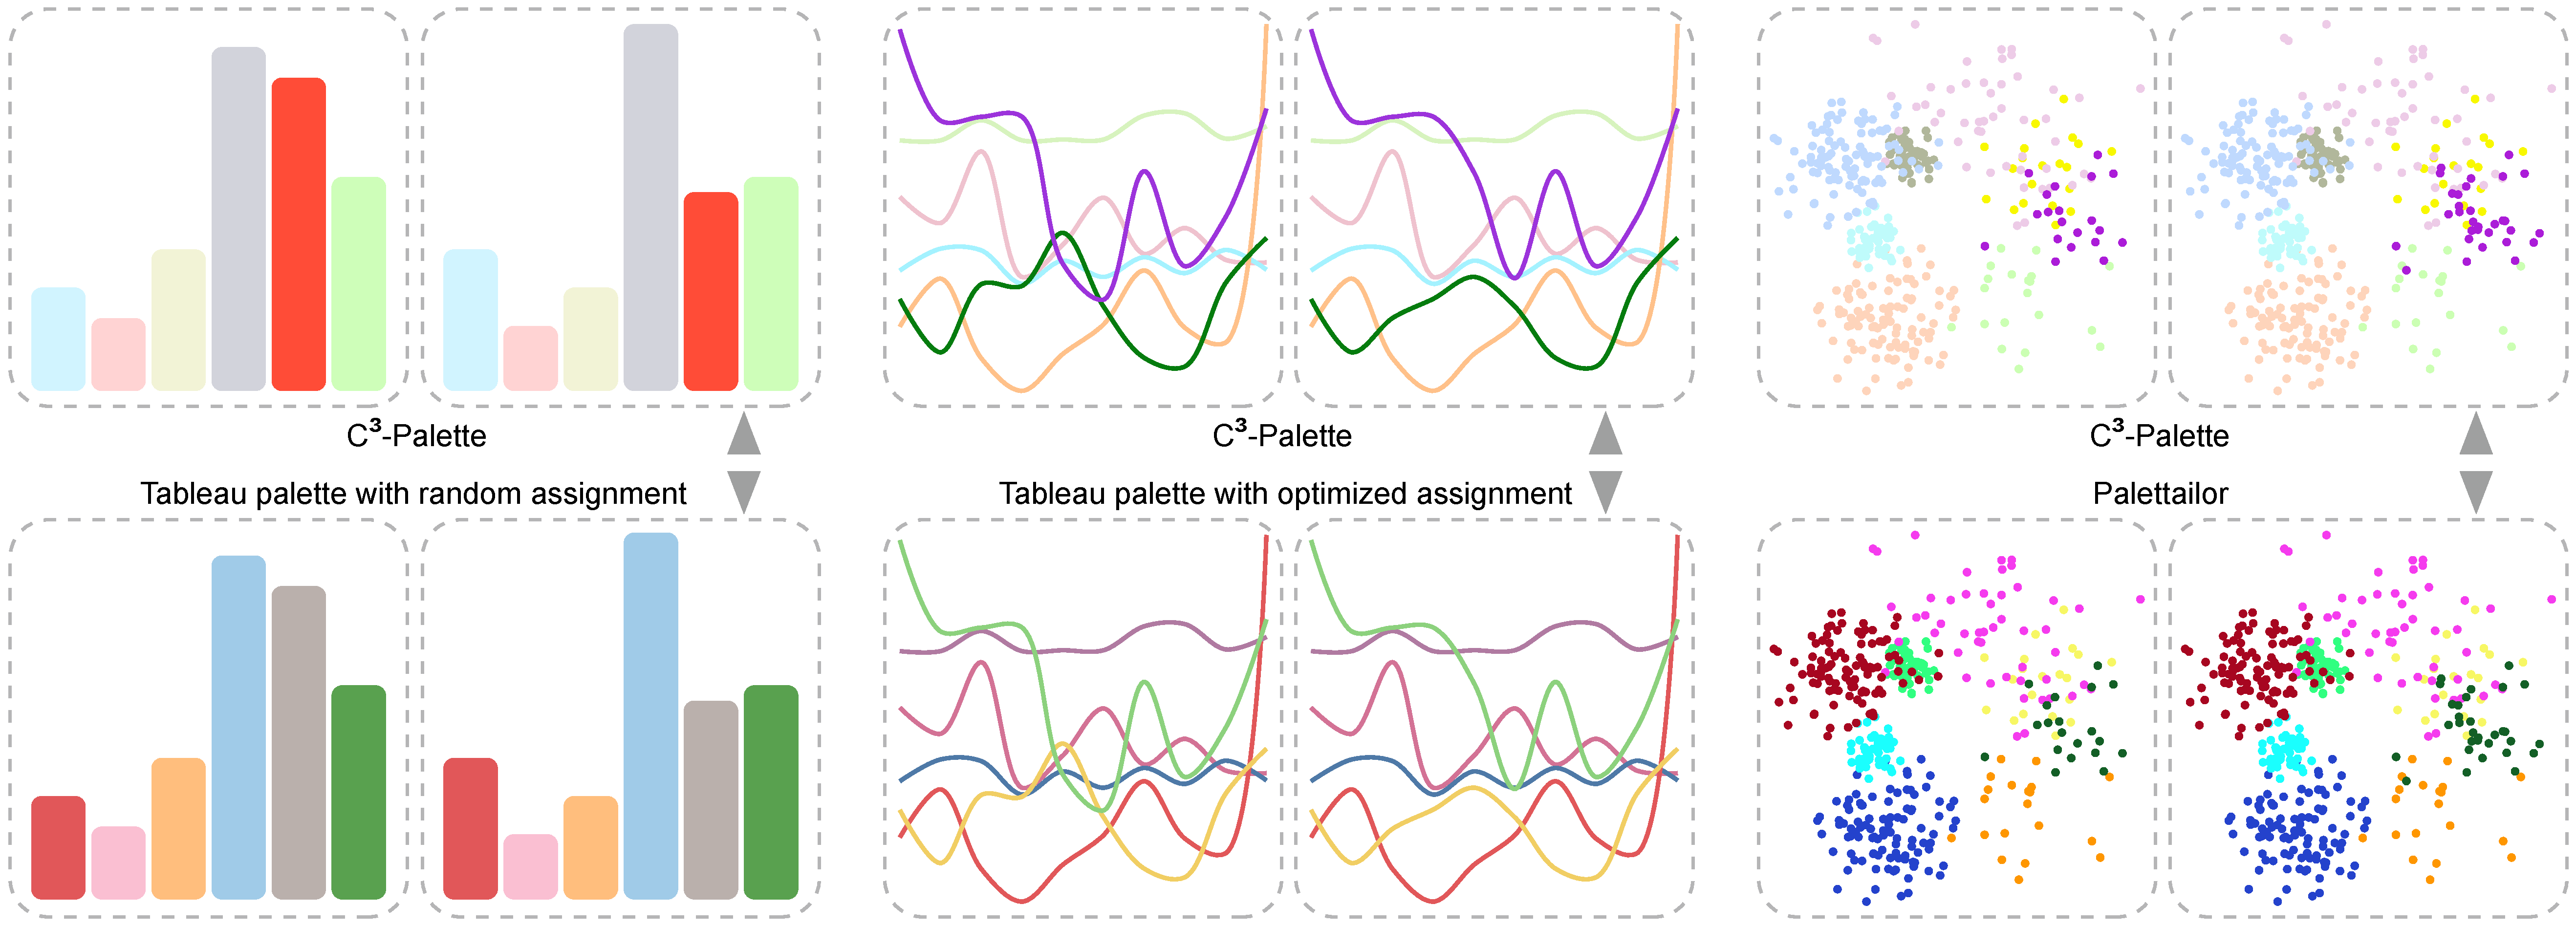
\includegraphics[width=\textwidth]{teaser6}
  \caption{
  Results for different types of categorical data visualizations: (left) $C^3$-palette versus Tableau palette with random assignment; (center) $C^3$-palette  versus
Tableau palette with optimal assignment; (right) $C^3$-palette versus Palettailor~\cite{Lu21}. Our co-saliency methods (top) can highlight the changed classes while
maintaining discrimination of classes.}
  \Description{Illustrating the different conditions used in the online experiment.}
  \label{fig:teaser}
\end{teaserfigure}

%%
%% This command processes the author and affiliation and title
%% information and builds the first part of the formatted document.
\maketitle

\section{Introduction}
Comparison is an indispensable task in data analysis and visualization. It often involves searching for categories (classes) with large or small changes among multiple categorical datasets.
%\footnote{The words ``labeled'' and ``categorical'' are interchangeable, and we study the quantitative data with a categorical variable.}.
Comparison are usually achieved through juxtaposition of multiple categorical visualizations~\cite{Gleicher18,LYi21} such as bar charts, line charts or multi-class scatterplots, where each category is commonly encoded by a unique color.
While color codings are known to play an important role in helping viewers see differences between juxtaposed views~\cite{Tominski08,Albers11,Gleicher18}, there is no color design scheme that optimizes visual comparisons, especially for the task of identifying the largest differences between charts~\cite{Ondov19}. %to ease the process for comparative visualization is a challenging and yet unexplored problem.

%For example, a market analyst
A typical scenario would be  a market analyst who uses comparisons to
%examines the annual and monthly profits of various products in these countries with bar and line charts, respectively. Using the product name for color encoding, he is able to  efficiently search the product with the largest differences from side-by-side \od{shown} bar and line charts.
investigate the performance of a company across different countries over the last couple years.
\od{S/he first would create a scatterplot for each year by showing the annual revenue and profit of each product by colorizing each point of the plot with a country label.
After finding the two countries with the largest changes, s/he then examines the annual and monthly profits of various products in these countries with bar and line charts. Using the product name for color encoding, s/he is able to  efficiently search the product with the largest differences from side-by-side shown bar and line charts}.


The most common way to colorize juxtaposed views is to manually find a color mapping for a    selected view while judging how well it fits to the other views. Such a trial and error procedure might converge to a desirable color mapping; however, the needed effort significantly increases with the numbers of classes and views. %whereas faceting classes into more views facilitates comparison of individual classes but requires too much space.
Although existing automated color selection approaches~\cite{Chen14,Wang2018,Lu21} allow to alleviate the effort for single view colorizations, the obtained color mapping might not be able to clearly reveal similarities or differences among multiple views. For example, the assignment of the Tableau palette for maximizing class separability \od{(cf. \cite{Wang2018})} in Fig.~\ref{fig:teaser}(center top) creates a visualization with better class discrimination, but the changed time series (see green and red curves in center bottom) are hard to identify.
Although such classes of interest could be highlighted by fading out background classes using alpha blending, this  inevitability would introduce visual ambiguities for overlapping classes~\cite{baudisch2004multiblending} and potentially lead to a poor class separation.
As far as we know, few existing visualization-oriented color selection tools (e.g., ColorBrewer~\cite{harrower2003colorbrewer} or Palettailor~\cite{Lu21}) allow for colorizing multi-view visualizations, let alone supporting comparisons in juxtaposed views.

%by juxtaposition.
%seeing differences between juxtaposed views.

%There are two simple ways to assist comparison task, one is using alpha-blending to highlight concerned classes, the other is using faceting by groups with the groups highlighted on top of all the cases~\cite{}\lk{These two are the alternatives the reviewer asked to compare.}. These two methods only cared about highlighting the concerned classes while make other classes invisible or hard to discriminate. However, user might want to explore one of the scatterplot. In this situation, alpha-blending need to set all classes' opacity back to 1.0 while facet need to show other classes to previous colors which might confuse people. As far as we know, there does not exist a method that unifies both highlighting important parts while maintaining good class separability for comparison task.

To fill this gap, we propose a comparison-driven color palette generation framework, which automatically generates appropriate color mappings for efficiently searching the largest \od{differences} from one categorical visualization to another.
To achieve this goal, we propose a co-saliency model to characterize the most salient features among juxtaposed categorical visualizations that are likely to attract visual attention. We borrow the idea from the concept of image co-saliency~\cite{Jacobs10}, which was originally designed for summarizing salient differences between two similar natural images.
%  by fusing image changes and single image saliency together.
% In line with this, we devise
Our co-saliency model allows to easily identify important features (e.g., changed classes) from juxtaposed categorical visualizations while maximizing the visual discrimination of classes in the individual visualizations. \od{It is achieved by fusing \od{two separate goals}: class importance between visualizations and class contrast within them.} Class contrast is based on perceptual separability \od{between}
% with
neighboring classes and with the background~\cite{Wang2018}, while
class \od{importance}
% change
is measured by summing up the changes of point positions and point numbers  of each class, where the position change is quantified by using the Earth Mover's Distance (EMD)~\cite{rubner2000earth}, a perceptual distance metric.
Classes with large importance and small class separability (strong overlap with other classes) are more co-salient, while classes with small importance or large separability (more compact) are less co-salient.

By integrating our co-saliency model into existing categorical data colorization tools~\cite{Lu21}, we can automatically generate color mappings that maximize co-saliency among juxtaposed visualizations. The resulting color mapping schemes let classes with large importance pop out from the context and will attract viewers' attention,  while at the same time maximizing the perceptual separability between classes in the individual visualizations. By doing so,
the major issue of a juxtaposition, that human have limited visual memory (see~\cite{Tominski12}), is greatly alleviated and visual searches can be performed with less cognitive costs~\cite{healey1995visualizing}.
%
The top of Fig.~\ref{fig:teaser} shows the results generated by our colorization method, where the changed classes pop out and can easier be spotted than the ones in the bottom of Fig.~\ref{fig:teaser}. Our results are similar to the ones of alpha blending, but still maintain the separability between classes due to the different hues.

 %of the class is further enhanced in Fig.~\ref{fig:teaser}(right bottom) by using our colorization method.
%Based on previous work~\cite{Wang2018, Lu21}, %we employ a carefully design for upward compatible. %That is, our method can be used for both single or multiple categorical visualizations. Thus
%we provide a unified framework for colorization, including automatic palette generation(like Lu et al.~\cite{Lu21}) for highlighting the classes with large delta between two data series, %and interactively highlighting  classes of interest %due to the importance factor which can be manually adjusted by user
%while maintains the class separability. Furthermore, users are allowed to highlight classes of interest by setting importance to them
%with the importance factor manually adjusted by user. %We also apply a color blindness simulator to generate palettes for people with color deficiency.

We evaluated our approach through carefully designed bar charts and scatterplots by comparing our colorized results with the ones produced by state-of-the-art palettes (e.g.,Tableau~\cite{tableau} and Palettailor~\cite{Lu21}). For bar charts, we replicated the experimental setting of Ondov et al.~\cite{Ondov19} but only performed the task of identifying a maximum \od{difference from two} horizontal juxtaposed bar charts, which is also referred as the MAXDELTA task by Ondov et al.~\cite{Ondov19}.
Next, we carried out studies with multi-class scatterplots generated by Lu et al.~\cite{Lu21}, whose counterparts were generated by changing the properties (point number and position) of several randomly selected classes.
\od{We first conducted a pilot study to verify the validity of our experimental setting and then ran two online studies: first, we investigated how well our generated palettes help users to identify changed classes of two scatterplots and second, we let them count class numbers in single scatterplots (discrimination task).
Lastly, we conducted a case study to demonstrate how our system helps comparing juxtaposed visualizations with multiple line charts.}
The results show that our approach is able to produce color mappings optimized for supporting comparison and aligned with the state-of-the-art palettes in maximizing perceptual class separability.

A web-based color design tool, \toolname-palette\footnote{\small \url{https://c3-palette.github.io/}}, named by \textbf{C}o-saliency based \textbf{C}olorization for \textbf{C}omparing multi-class scatterplots, allows to show coordinated views and let users  explore the relationship between multiple data sets with different color mapping schemes.
%Inspired by volume visualization~\cite{kindlmann1998semi}, we provide a transfer function view for users to highlight different classes of interest.
%First, users can specify some classes of interest like the ones with subtle differences and our approach can generate  color mappings with the maximized co-saliency for these classes.
%Second, users might prefer specific colors for some classes based on semantics and accordingly our approach generates color mapping schemes that meet these constraints.
%Third, our approach can work in a reverse way that can generate a color mapping scheme to highlight the classes with less changes while obscuring the ones with large changes.
%Last, we extend our method to colorize small multiples like scatterplot matrices by integrating the spatial proximities between views
The main contributions of this paper are as follows:
%\vspace*{-2mm}
\begin{itemize}[noitemsep]
\setlength{\itemsep}{5pt}
  \item We propose a multi-class data visualization co-saliency model for measuring the importance of each data item shown in juxtaposed visualizations and use this metric to automatically generate color mapping schemes for effective comparisons;
  %\vspace*{-1mm}
    \item
  We provide an interactive tool that demonstrates how our approach can be used for visually comparing categorical visualizations or highlighting important classes within single scatterplots; and
  \item
   We evaluate the effectiveness of the resulting color mapping schemes in supporting both, visual comparison and visual discriminability, with three online user studies and a case study (Section~\ref{sec:results}).

  %\ms{I am not sure if categorical visualizations and categorical data is the right terminology to be used here. The data that we are working with is primarily quantitative with an additional variable (class label) that we use for color coding.  I personally feel like labeled data would be a better fit, or data with a categorical variable, but the latter is a bit long. Please pick one that you like and change the paper so the usage is consistent. I will not change further appearances of that, as this first needs a decision.  }
\end{itemize}
%\ms{general comment:  should \toolname~only refer to the webtool or to our technique.  I feel the later would be nicer. }

% Comparing multiple categorical datasets is a frequent task in visualization: trend tracing~\cite{Robertson08}, XX~\cite{} and XX~\cite{} are all examples.
% Different to single categorical data, however, the goal of visualizing multiple categorical data is not only to discriminate multiple categories, but also looking for changes from one set to another~\cite{Robertson08,Ondov19}.
% Both class discriminability and change perception are strongly influenced by the assigned colors~\cite{Tominski08,Lee13,Zhou16}. However, designing an appropriate a set of colors for multiple categorical datasets are tedious and time-consuming, especially when the number of categorical datasets and categories becomes higher.

\section {Related Work}
We begin by reviewing previous work related to visual comparison, color design for visualization, and
visual saliency/co-saliency.


\subsection{Visual Comparison}
Visual comparison is an essential part of interactive data analysis, which is regarded as a high-level ``compound task.'' Gleicher et al.~\cite{Gleicher11} provide a systematic review of techniques developed for better supporting comparison and summarize three basic layout designs for comparative visualization, including \emph{juxtaposition}, \emph{superposition} and \emph{explicit encoding}. Among them, juxtaposition places different datasets in different views without any change to the original visualization design and thus it is commonly used in many applications~\cite{munzner2003treejuxtaposer,Albers11,Lobo15}. However, it often causes cognitive burden because users need to maintain a mental image of one view for comparing with another view~\cite{LYi21}. Recently, Ondov et al.~\cite{Ondov19} and Jardine et al.~\cite{jardine2019perceptual} evaluated the perceptual effectiveness of different layouts for bar charts comparison with a few low-level tasks, which show that juxtaposition is less effective in some tasks like finding ``biggest delta between items.''
Accordingly, Gleicher et al.~\cite{Gleicher11} and  L'Yi et al.~\cite{LYi21} both suggested to carefully design visual encoding for improving its effectness. Our method facilitates visual comparison of categorical data by improving the visual search with the pop-out effect~\cite{enns1990three} induced by our proposed color mapping scheme.


\subsection{Color Design}
%Creating an appropriate color mapping scheme is crucial for data visualization and has attracted considerable attention.
For a complete review of color design for visualization, we refer readers to survey papers~\cite{Tominski08,Zhou16}. We limit our discussion to the techniques related to color design for categorical data visualization including color mapping optimization, color palette generation, and color design for multi-view visualization.

\vspace{1.5mm}
\noindent\textbf{Color Mapping Optimization}. Mapping each class to a proper color selected from the given palette is particularly helpful for categorical data visualization. %\footnote{The word ``proper'' means that the color mapping can help user discriminate each class.}
A few different factors have been used for guiding the search of such mappings.
For example, Lin et al.~\cite{lin2013selecting} proposed to optimize the compatibility between the class semantics and the assigned colors. Setlur and Stone~\cite{setlur2016linguistic} produced better results by using co-occurrence measures of color name frequencies.
For the classes without clear semantics,  Hurter et al.~\cite{Hurter10} suggested to maximize perceptual color differences among close lines of a metro map.
Kim et al.~\cite{Kim14} incorporated color aesthetics and color contrast into the optimization of color assignment for image segments.
Recently, Wang et al.~\cite{Wang2018} proposed to maximize class discriminability based on color-based class separability, which takes into account spatial relationships between classes and the contrast with background color.
Once an assignment is specified, the color for each class can be further optimized to better serve different purposes, such as reducing power consumption of displays~\cite{chuang2009energy} ,
improving the accessibility of visualizations for visual impaired users~\cite{machado2009physiologically}, and better class discrimination~\cite{lee2013perceptually}.
Almost all these methods aim to generate effective visualizations for single data, whereas our goal is to efficiently visualize salient class differences across multiple similar datasets with the same label information. One example is the instances of the same datasets evolving over time.
% \ms{along similar lines as before: You often say comparing different data sets. Imho that is bit too generic as for different datasets we usually cannot assume I direct mapping between points and classes. In stead, I think of it as changing instances of the same datasets. E.g. when changing over time. Please do fix that.}

\vspace{1.5mm}
\noindent\textbf{Color Palette Generation}.
%Rather than restricting the colors provided by the selected palette, the technique of color palette generation is to select colors from the color space.
To have an appropriate categorical color palette, the commonly used approach is to select from
a library of carefully designed palettes provided by online tools (e.g. ColorBrewer~\cite{harrower2003colorbrewer}).
Colorgorical~\cite{Gramazio17} further allows users to customize color palettes by generating palettes based on user-specified discriminability and preference importance.
Chen et al.~\cite{Chen14}  suggested to directly search proper colors in CIELAB space for maximizing class discrimination in multi-class scatterplots. Yet, it cannot find enough colors with large color differences, because of leaving out L* channel in the optimization.
Recently, Palettailor~\cite{Lu21} takes a further step that can automatically generate categorical palettes for different types of charts, such as scatterplots, line and bar charts.
All the aforementioned methods deal with single data, while our work focuses on visual comparison of multiple similar labeled datasets with some changed instances.

\vspace{1.5mm}
\noindent\textbf{Multi-view Color Design}.
Multi-view visualizations are commonly used in multivariate analysis. Although a few design guidelines~\cite{wang2000guidelines} have been proposed for constructing multi-view visualizations, few of them are related to color design. Qu et al.~\cite{qu2017keeping} recommended a set of color consistency constraints across views.
Among them, the high level constraint that the same data field should be encoded in the same way is related to our studied comparative visualization. Namely, all juxtaposed views should have the same color mapping scheme and a good scheme can help for seeing the differences between views.
However, few work has been done for finding such schemes. The only exception is comparing multiple continuous scalar fields~\cite{Tominski08} with an improved global color map by merging overlapping value ranges in different datasets. Our work is the first to generate appropriate color mapping for comparing multiple categorical visualizations.



\subsection{Visual Saliency \& Co-saliency}
Here we briefly review the visual saliency model developed for visualizations and image co-saliency models.

\vspace{1.5mm}
\noindent\textbf{Saliency for Visualization}.
The human visual system enables viewers to concentrate on salient regions of an image while ignoring the others. It is guided by two major factors~\cite{connor2004visual}: pre-attentive, bottom-up attention based on visual features (e.g., color, intensity and edges) and task-driven, top-down attention based on prior knowledge. %whereas the regions identified by these factors might be inconsistent in some cases.
A numerous of saliency models~\cite{borji2019salient} have been developed to mimic bottom-up attention mechanism in computer vision community.
Most of them model image saliency as the contrast of image regions to their surroundings with low level features. Among them, the most influential one is the Itti model~\cite{Itti98}, which computes image saliency with central surrounded differences. Kim et al.~\cite{Kim06} tailored this model to increase the visual saliency of selected regions of a volume dataset.  J$\ddot{a}$nicke and Chen~\cite{Janicke10} employed this model~\cite{Itti98} to define a quality metric for evaluating visualizations.
Recently, Matzen et al.~\cite{Matzen18} evaluated a variety of saliency models on a large visualization dataset and explored why these models work poorly for visualization images. One major reason is that visualizations are often created for specific goals, whereas existing models are based on the bottom-up attention. To overcome these weaknesses, they proposed a data visualization saliency (DVS) model by incorporating meaningful high-level text features into Itti's model. However, this model is not designed on the class-level and cannot be directly used for categorical visualizations.

%All these models assess the quality of single images without the consideration of data analysis tasks, while our goal is to develop a model for better serving the task of visual comparison.


%
\vspace{1.5mm}
\noindent\textbf{Image Co-Saliency}.
Unlike single image based saliency model, the co-saliency model estimates the saliency (importance) of each pixel within the context of multiple related images. Jacobs et al.~\cite{Jacobs10} developed the first co-saliency model for highlighting the most salient differences between two compared images.  Later, this concept has been extended for discovering common and salient objects/foregrounds from image collections~\cite{zhang2018review}. Inspired by the original model~\cite{Jacobs10}, our work attempts to design an appropriate color mapping for visualizing the most co-salient features among juxtaposed labeled data visualizations. Following their findings that the co-salient features can be effectively characterized by fusing image changes and single image contrast together, our co-saliency model relies on two factors: the class contrast in individual views  and global features from in-between views (e.g., class structure changes).

\section{Co-Saliency based Color Design}
Given $N$ ($N\geq 2$) categorical visualizations with the same class labels (or a subset thereof), the $j$th visualization has $M$ classes and $n_j$ data items $\{\mathbf{x}^j_1, \cdots, \mathbf{x}^j_{n_j}\}$, where each $\mathbf{x}^j_t$ has a label
$l(\mathbf{x}^j_t)$ and the $i$-th class (with $n^j_i$ data points) consists of $\{\mathbf{x}_{i,1}^j, \cdots , \mathbf{x}_{i,n^j_i}^j\}, i \in  \{ 1, \cdots, m \} $.
For standard bar and line charts, $M$ is equal to $n_j$ but it is often smaller than $n_j$ for scatterplots.
All visualizations use the same  background color $\mathbf{c}_b$ and the same color mapping scheme $\tau: L \mapsto c$. Our goal is to find the best mapping $\tau$ that supports an effective comparison of multiple categorical \od{visualizations}.
% scatterplots.

In line with the design requirements for natural image comparison and categorial data visualization~\cite{Jacobs10,Gleicher18,Lu21},
%~\cite{itti1998model,cheng2014global,zhang2018review},
our problem is formulated based on the following three design requirements:
\begin{enumerate}[label=(\roman*),nosep]
\item \textbf{DR1:} highlighting the most concerned classes between visualizations as much as possible for an efficient comparison;
\item \textbf{DR2:} maximizing the visual discrimination between classes in the individual visualizations for an efficient exploration of multi-class data; and
\item \textbf{DR3:} providing flexible interactions for the exploration of relationships among the compared datasets.
%co-salient classes should follow the principles of visual salience in individual visualizations so that the co-salient classes can be easily identified.
\end{enumerate}
Although visual comparison is an essential part of interactive data analysis, most of  the existing  colorization techniques~\cite{Gramazio17, Lu21} attempt to meet DR2. The key challenge in meeting DR1 is that we need a proper model to characterize the most salient features in multiple visualizations.
To address this issue, we propose our %a categorical visualization
co-saliency model that calculates the saliency of each data item in the context of other similar visualizations. Integrating this model into the objective of a state-of-the-art color mapping generation framework~\cite{Lu21}, we can
generate proper color mappings that highlight salient differences between juxtaposed categorical visualizations while fostering a better visual discrimination of classes.

\subsection{Co-saliency for Multi-class Scatterplots }
Following the definition of image co-saliency~\cite{Jacobs10}, we model class co-saliency with two factors: class importance between visualizations and class contrast within visualizations. The class importance describes how much each class should stand out from the visualization.
Class contrast describes how much each class stands out from neighboring classes and the background,
which is similar to perceptual class separability~\cite{Aupetit02,Wang2018}. Hence,
we define two types of class contrasts: a local contrast with neighboring classes and a contrast with the background.

Since point-based representations are very general in 2D visualization, we use two ($M=2$) horizonally juxtaposed scatterplots to illustrate our method.
Analogous to bottom-up image co-saliency models~\cite{Jacobs10,Fu13}, the co-saliency of the $i$th class is defined as the product between the class importance and  class contrast scores to emphasize the target class and the co-saliency for $M$ classes:
\begin{equation}
% E_{CoS} = \sum_i   \sum_j (1-\lambda) \alpha^j_i  \exp(\theta_i) + \lambda \beta_i  f(\theta_i)
E_{CoS} = \sum_i^M    \left(\sum_j^N \frac{1}{n^j_i}\bigg(\lambda \alpha^j_i\exp(\theta_i) + (1-\lambda) \beta^j_i f(\theta_i) \bigg) \right)
	\label{eq:cosaliency}
\end{equation}
where $\theta_i$ is the importance of the $i$th class,
$n^j_i$ is the number of points of the $i$th class in the $j$th scatterplot,
$\alpha^j_i$ is the local contrast with the neighboring classes of the $i$th class in the $j$th scatterplot, $\beta^j_i$  is the contrast of the class to the background, and $\lambda$ is the weight between them. The weight $1/{n^j_i}$  is used to alleviate class imbalances  so that  classes with small numbers of points and large changes can be highlighted.

To better support DR1, we apply an exponential function to enlarge the weight of structural class changes, while using a piecewise function weighting the background contrast:
\begin{align}
f(\theta_i) =  \left\{ \begin{array}{ll}
\exp(\theta_i) & \textrm{if $\theta_i>\kappa$}\\
-\exp(\theta_i) & \textrm{else}
\end{array} \right.
\label{eq:energyfunc}
\end{align}
$\kappa$ is a user-specified threshold with a default of zero. The reason for the two different weighting schemes is that classes with less or no changes might be treated as the background by viewers~\cite{zhang2018review}. To suppress the saliency of such classes, we introduce a negative importance for them.

\vspace{2mm}
\noindent\textbf{Local Contrast}.
%Given the $j$th scatterplot, we define the local class contrast based on the point distinctness~\cite{Lu21}.
%Here, we briefly describe its computation process and
%refer to Lu et al.~\cite{Lu21} for more details.
%Given the data point $\mathbf{x}^j_t$, its distinctness is defined as the sum of the color differences from its neighbourhoods weighted by the inverse Euclidean distance.
%Then, the distinctness of the $i$th class is the sum of all points with the same class label in the scatterplot, which is further normalized by ${n^j_i}$.
Given the $j$th scatterplot, we define the local class contrast based on the $\alpha$-shape based point distinctness~\cite{Lu21}.  For each data point $\mathbf{x}^j_t$, we define its point distinctness  as:
\begin{align}
 \gamma (\mathbf{x}^j_t)=\frac{1}{|\Omega^j_t|} \sum_{\mathbf{x}^j_p \in \Omega^j_t}  \frac{\Delta\epsilon(\tau(l(\mathbf{x}^j_t)),\tau(l(\mathbf{x}^j_p)))}{d(\mathbf{x}^j_t,\mathbf{x}^j_p)} \nonumber ,
\end{align}
where $\Omega^j_t$ is set of $k$ nearest neighbors of $\mathbf{x}^j_t$, $\tau(l(\mathbf{x}^j_p))$ is the color of $\mathbf{x}^j_p$,  $d$ is the Euclidean distance and $\Delta\epsilon$ is the CIELAB color distance.
For the $i$th class, its local contrast is the sum of all points with the same class label in the scatterplot:
\begin{align}\label{eq:nc}
 \phi^j_i = \frac{1}{n_j}\sum^{n_j}_{p}\gamma(\mathbf{x}^j_p) \delta(l(\mathbf{x}^j_p),i)
\end{align}
where $\delta(l(\mathbf{x}^j_p),i)$ is one if the class label $l(\mathbf{x}^j_p)$ is $i$ and else zero.

If a class overlaps with different classes, the local contrast value will be high and the value will be small for a well separated class. Hence, the black class  in the  two scatterplots shown in Fig.~\ref{fig:map}(a)  has a low contrast value (see Fig.~\ref{fig:map}(b)) and the cyan class has a large value.


%\begin{align}\label{eq:pdc}
% \alpha^j_i = \frac{1}{n^j_i}\sum^{n_j}_{p}\gamma(\mathbf{x}^j_p) \delta(l(\mathbf{x}^j_p),i)
%\end{align}
%where $\delta(l(\mathbf{x}^j_p),i)$ is one if the class label $l(\mathbf{x}^j_p)$ is $i$ and else zero.
%
%
%However, KNNG cannot reflect the contrast among classes without any overlap. For example,  in Fig.~\ref{fig:knng}(a) the contrast between the blue class and the brown classes cannot be reflected.
%To address this issue, we introduce an additional class-center based contrast cue~\cite{Fu13}.
%Suppose the center of the $i$th class in this scatterplot is $\mu^j_i$, the class contrast is:
%\begin{align}\label{eq:cc}
% \varphi^j_i =  \frac{1}{M}\sum^M_{m}\frac{\Delta\epsilon(\tau(i),\tau(m))}{||\mu^j_m -\mu^j_i ||},
%\end{align}
%which assigns large weights to nearby classes and small ones to far-away classes. The final class contrast of the $i$th class is:
%\begin{align}\label{eq:pd}
% \alpha^j_i  = \phi^j_i  + \omega \varphi^j_i,
%\end{align}
%where the weight $\omega$ is 1.0 in our experiment.

\vspace{2mm}
\noindent\textbf{Background Contrast}.
The contrast with the background is based on the \od{so-called} point non-separability $\rho (\mathbf{x}^j_t)$ (rf.~\cite{Wang2018}), which is defined as the difference between two  separation degrees:
\begin{align}
\rho(\mathbf{x}^j_t)&= b(\mathbf{x}^j_t)-a(\mathbf{x}^j_t) \ .
\end{align}
where $b(\mathbf{x}^j_t)$ is the between-class separation degree and $a(\mathbf{x}^j_t)$ is the within-class separation degree.
% of $\mathbf{x}^j_t$.
\od{The measures are defined as weighted sums of  color differences of $\mathbf{x}^j_t$ with its neighborhood from the same and different classes:}
\begin{align}
a(\mathbf{x}^j_t)&=\frac{1}{|\Omega^j_t|}\sum_{\mathbf{x}^j_p \in \Omega^j_t } \frac{\delta(l(\mathbf{x}^j_t), l(\mathbf{x}^j_p))
\Delta\epsilon(\tau(l(\mathbf{x}^j_t)),\mathbf{c}_b)
}{d(\mathbf{x}^j_t,\mathbf{x}^j_p)} , \;\;
b(\mathbf{x}^j_t)=\frac{1}{|\Omega^j_t|}\sum_{\mathbf{x}^j_p \in \Omega^j_t } \frac{1-\delta(l(\mathbf{x}^j_t), l(\mathbf{x}^j_p))\Delta\epsilon(\tau(l(\mathbf{x}^j_t)),\mathbf{c}_b)}{d(\mathbf{x}^j_t,\mathbf{x}^j_p)}  \nonumber
\end{align}

When most neighbor points of $\mathbf{x}^j_t$ have the same label as $\mathbf{x}^j_t$,  $\rho (\mathbf{x}^j_t)$ is negative.
% and vice versa.
%the corresponding class has large within-class separability and small between-class separability and thus $\rho (\mathbf{x}^j_t)$ is negative; and vice versa.
However, such a negative $\rho (\mathbf{x}^j_t)$ makes the optimization in Eq.~\ref{eq:cosaliency} meaningless, \od{and the corresponding} classes might be highlighted no matter how large the change of this class is.
\od{To address this issue, we use an exponential function to let $\rho (\mathbf{x}^j_t)$  always be positive while maintaining the monotonicity of the function.} Accordingly, we define
%\begin{align}\label{eq:ctb}
% \rho (\mathbf{x}^j_t)=\frac{1}{|\Omega^j_t|} \sum_{\mathbf{x}^j_p \in \Omega^j_t}  \frac{(1-2\delta(l(\mathbf{x}^j_t),l(\mathbf{x}^j_p)))\Delta\epsilon(\tau(l(\mathbf{x}^j_t)),\mathbf{c}_b)}{d(\mathbf{x}^j_t,\mathbf{x}^j_p)} ,
%\end{align}
the contrast to the background of the $i$th class as:
\begin{align}\label{eq:ctbc}
 \beta^j_i = \frac{1}{n^j_i}\sum^{n_j}_{t} \exp(\rho(\mathbf{x}^j_t)) \delta(l(\mathbf{x}^j_t),i).
\end{align}
%where
%$\delta(l(\mathbf{x}^j_p),i)$ is one if the class label $l(\mathbf{x}^j_p)$ is $i$ and else zero.
%In doing so, all classes have positive background contrast value.
As illustrated in Fig.~\ref{fig:map}(c), well-separated classes with large color differences from the background have large background contrast (blue and black classes), whereas the pink and cyan classes have relatively large background contrast values with a medium class separation.


%\begin{wrapfigure}{r}{0.28\columnwidth}
%	\vspace{-5mm}
%	\centering
%	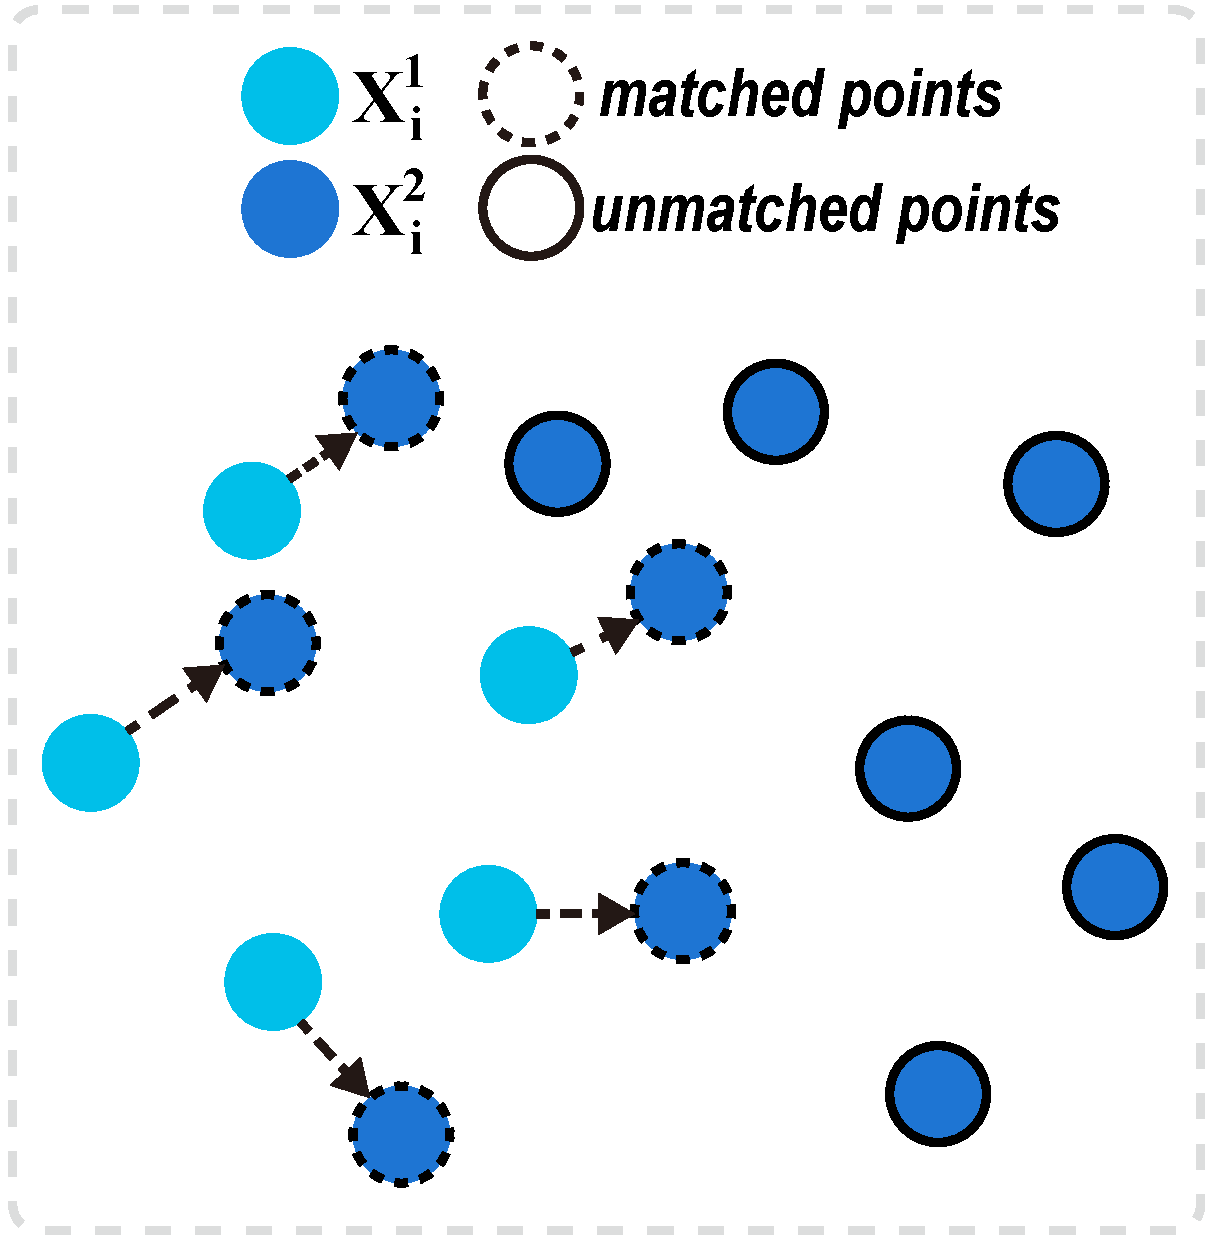
\includegraphics[width=0.28\columnwidth]{class-change-degree}
%	\vspace*{-8mm}
%	\caption{An one-to-one mapping for computing the changes between two classes.}
%	\vspace*{-2mm}
%	\label{fig:class-change-degree}
%\end{wrapfigure}
 %Since $\rho (\mathbf{x}^j_t)$ might be a negative value which will be influenced by Eq.~\ref{eq:piecewiseFunc}, we apply an exponential function to transfer it to positive while maintains the monotonicity.

\vspace{1.5mm}
\noindent\textbf{Class Importance}.
Class importance reflects whether a class should be highlighted or not. It can be specified by user or by some measures. In our paper, as a default we use the class change degree to represent the importance of each class.
To quantify how users perceive structural changes of classes, we measure the difference between the class distributions in two scatterplots using the Earth Mover's Distance (EMD)~\cite{rubner2000earth}, a perceptual metric.
Suppose the $i$th  class with two \od{representations by two} sets of points $\mathbf{X}^1_i = \{\mathbf{x}_{i,1}^1, \cdots , \mathbf{x}_{i,n^1_i}^1\}$ and $\mathbf{X}^2_i = \{\mathbf{x}_{i,1}^2, \cdots , \mathbf{x}_{i,n^2_i}^2\}$.
Taking the Euclidian distance between points as the cost, we need to  minimize the total matching cost
\begin{align}
 H(\mathbf{X}^1_i, \mathbf{X}^2_i)  = \min_\chi \sum_t d(\mathbf{x}_{i,t}^1, \mathbf{x}_{i,\chi(t)}^2), \nonumber
\end{align}
which constrains one-to-one mappings $\chi$ between points %(see an illustration in Fig.~\ref{fig:class-change-degree}).
This is the classic bipartite matching problem, which can be solved by the Hungarian method~\cite{kuhn1955hungarian}.
When the number of points of two sets is not equal, we further take the difference between the number of points into account. \od{In doing so, the class change degree contains  positional changes and changes of element numbers:}
\begin{align}\label{eq:cm}
 \theta_i= \frac{H(\mathbf{X}^1_i, \mathbf{X}^2_i) }{\min\{n^1_i, n^2_i\}} + \nu \frac{||n^1_i- n^2_i||}{\max\{n^1_i, n^2_i\}}
\end{align}
both terms range within [0,1] and $\nu$ is 1.0 as default value.


\begin{figure*}[!tb]
\centering
\includegraphics[width=\linewidth]{figures/saliencymap}
\caption{Main components for computing co-saliency maps: For the two input scatterplots (a), our class-based co-saliency (e) is generated by fusing  local contrast (b),  background contrast (c),  and class change degree (d). Brightness of points denotes value.
	% and vice versa.
}
\vspace*{-3mm}
\label{fig:map}
\end{figure*}
\vspace{1.5mm}

Fig.~\ref{fig:map} shows an example of two 8-class scatterplots with three  changing classes (orange, blue and black). Combining the class change degree with the two above-given contrast measures allows us to highlight salient differences and maintain the visual discrimination of the classes (see Fig.~\ref{fig:map}(e)).

\subsection{Co-Saliency based Color Mapping}
\label{subsec:solver}
On the basis of the co-saliency model, we meet DR1 and DR2 in two ways: co-saliency based color assignment and co-saliency based palette generation.

\vspace{1.5mm}
\noindent\textbf{Co-saliency based Color Assignment}.
Given a good color palette with $P$ colors ($P\geq M$), the optimal color mapping can be obtained by
taking the co-saliency model in Eq.~\ref{eq:cosaliency} as the objective of the state-of-the-art color assignment method~\cite{Wang2018}. Starting from a random permutation of $P$ colors, we use the simulated annealing algorithm~\cite{aarts1989stochastic} to find the optimal permutation with two randomized strategies to improve the solution. One is randomly exchanging two colors from the selected $m$ colors and the other is replacing one color from the $m$ selected colors with the one chosen from the unselected $P-M$ colors. With a few iterations, we can obtain a reasonable color mapping as shown in Fig.~\ref{fig:teaser} bottom left.

\begin{figure}[h]
\centering
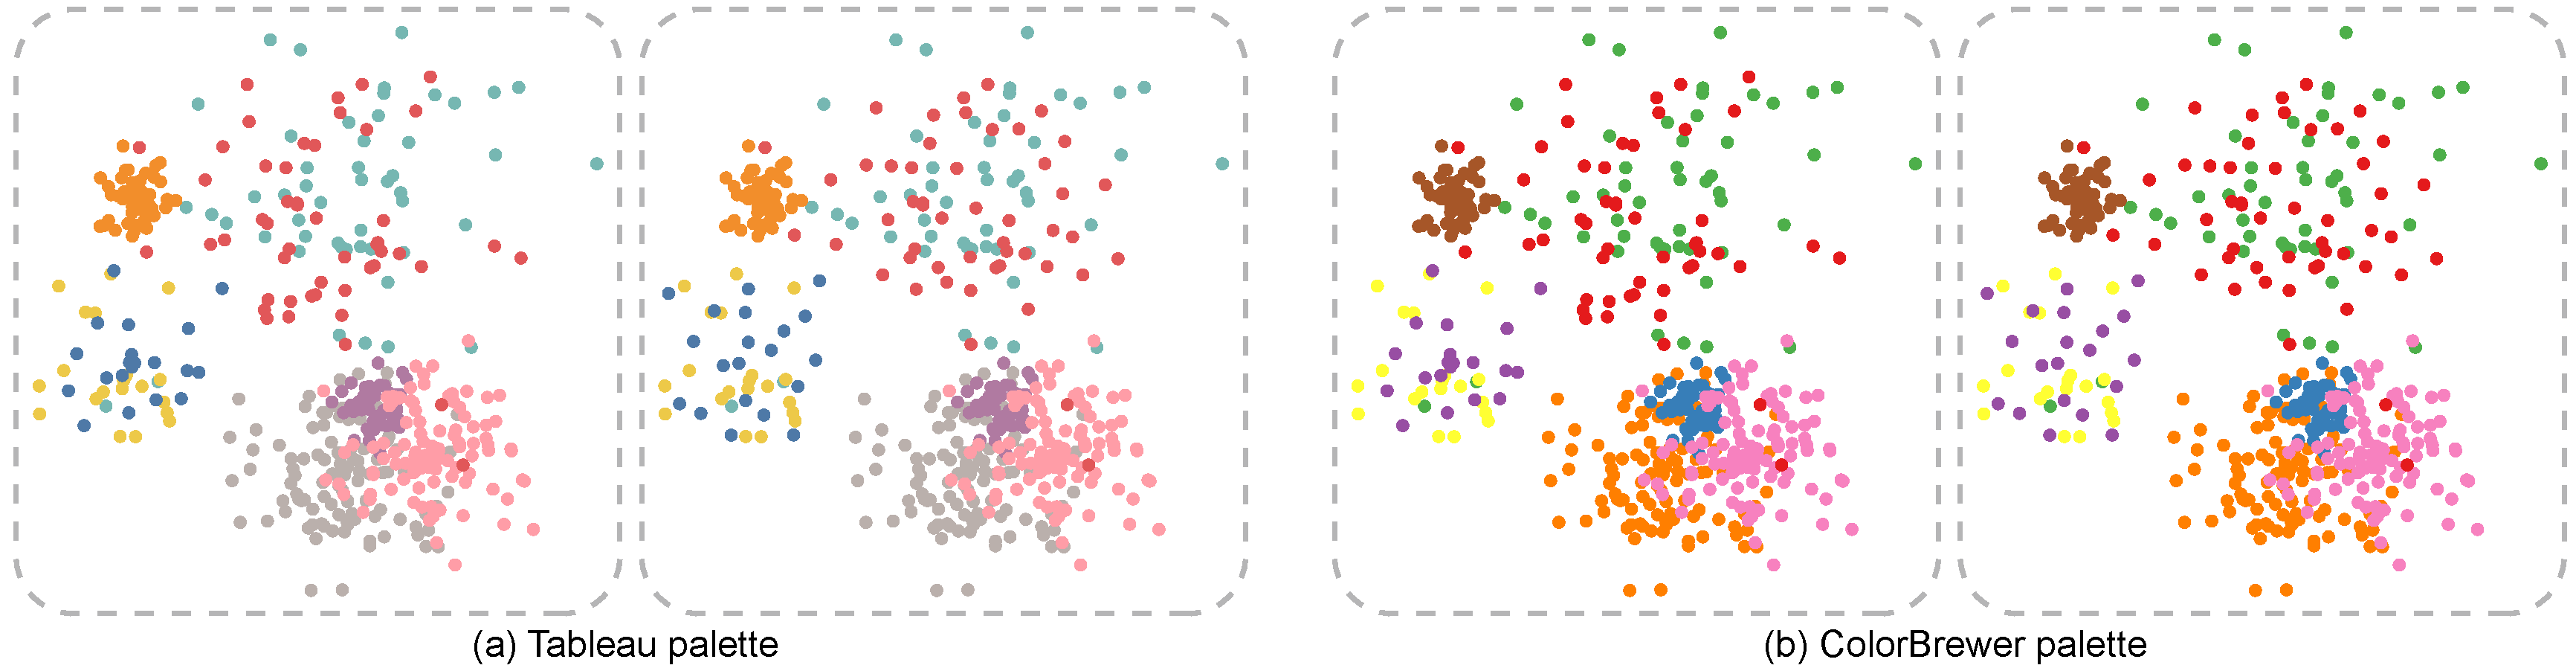
\includegraphics[width=.8\columnwidth]{figures/colorbrewer.pdf}
\caption{Visualizing the same data sets as shown in Fig.~\ref{fig:lambda} with the ColorBrewer palette and our assignment method.}
\vspace*{-3mm}
\label{fig:colorbrewer}
\end{figure}

However, this method has two major limitations: i) requiring users to try many palettes for selecting a good one; and ii) the design of most existing palettes is not oriented towards visual comparison so that even the best color assignment cannot provide prominent cues for this task.
%For example, all colors in the Tableau palette are highly discriminable and it is hardly to find a satisfactory solution, see Fig.~\ref{fig:teaser} (b). Thus, we prompt users to use our co-saliency based palette generation method.
For example, all colors in the ColorBrewer 8-class Set1~\cite{harrower2003colorbrewer} palette are highly discriminable, but it is hard to find a satisfactory solution. Fig.~\ref{fig:colorbrewer} shows an example, where the change of the red class is hard to identify at once even it is very distinctive. Thus, we prompt users to use our co-saliency based palette generation method.


\vspace{1.5mm}
\noindent\textbf{Co-saliency based Palette Generation}.
The recently proposed data-aware palette generation method~\cite{Lu21} automatically generates discriminable and preferable palettes by maximizing the combination of three palette quality measures: point distinctness, name difference, and color discrimination.
By replacing the first measure with our co-saliency model, the palette generation is formulated as an optimization problem:
\begin{equation}
\arg\max_{\mathbf{\tau}} E(\mathbf{\tau}) = \omega_0 E_{CoS} + \omega_1 E_{ND} + \omega_2 E_{CD}.
\label{eq:energyfunc}
\end{equation}
which consists of a co-saliency term $E_{CoS}$ (see Eq.~\ref{eq:cosaliency}), a name difference term $E_{ND}$ and a color discrimination term $E_{CD}$, balanced by $\omega_0$, $\omega_1$ and $\omega_2$. For more detail about $E_{ND}$ and $E_{CD}$, we refer readers to~\cite{Lu21}. By using the same optimization method as Lu et al.~\cite{Lu21}, we can generate desired colors in real time. %see Fig.~\ref{fig:teaser} (d).



\subsection{Parameter Effect}
\label{subsec:parameter}
Besides different weights for different terms in palette generation~\cite{Lu21}, our co-saliency model involves three parameters: the weight $\lambda$ between two contrasts, the threshold for the class importance $\kappa$, and $\nu$ that is related to the definition of the class change degree which is used as our default class importance.
Since $\nu$ is fixed in our experiments and the class importance can be specified by user, we mainly discuss the effects of $\lambda$  and $\kappa$.

\begin{figure}[h]
\centering
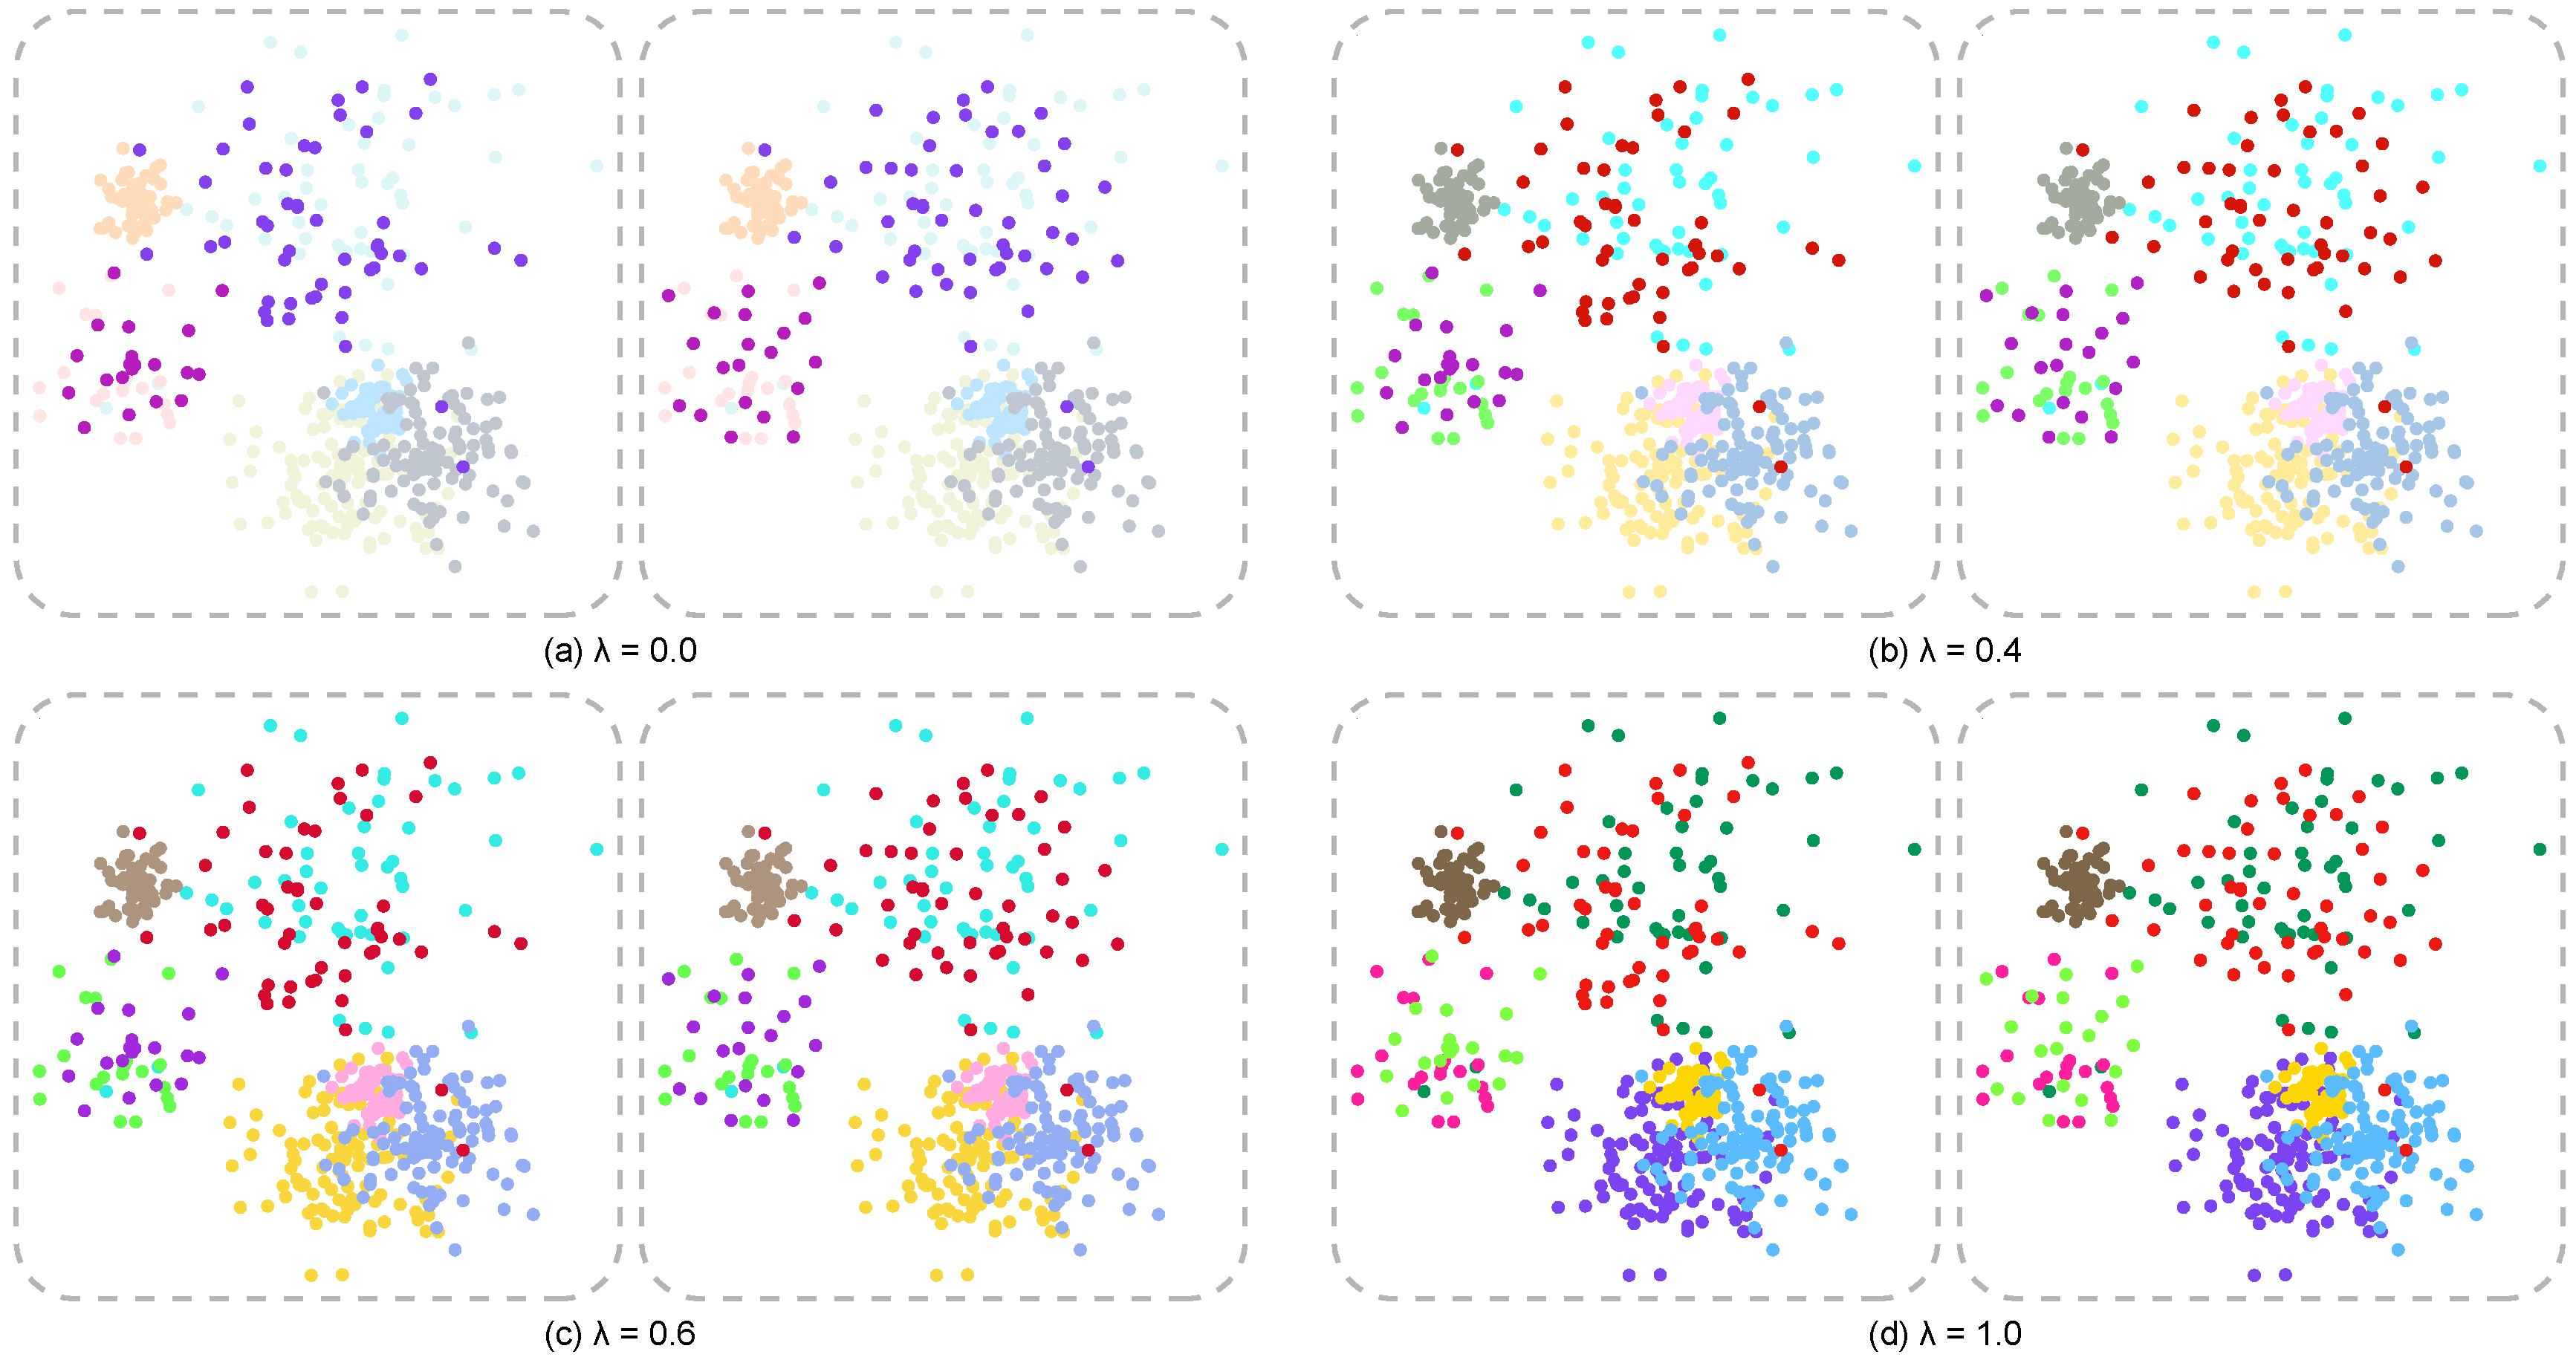
\includegraphics[width=0.8\textwidth]{figures/lambda.pdf}
\caption{Effect of $\lambda$: (a) result generated by only considering contrast to the background; (b) result generated by setting $\lambda$ to 0.4; (c) result generated by setting $\lambda$ to 0.6; (d) result generated by only considering contrast with nearest classes.}
\vspace*{-3mm}
\label{fig:lambda}
\end{figure}
%\vspace{3mm}

\noindent\textbf{Balancing Weight $\lambda$}.
Although this parameter modulates the influence between the class contrast with neighbors and background, it offers a compromise between DR1 and DR2.
As shown in Fig.~\ref{fig:lambda}(a), considering only the contrast to the background would have a good 'pop out' effect but other classes are hard to discriminate. While considering only the contrast with nearest neighbors, such as Fig.~\ref{fig:lambda}(d), all the classes are each to distinguish but the changed classes are hard to find out.
This is reasonable, because pre-attentive vision
% processing mechanism
lets a bright saturated color region within  regions of de-saturated colors ``pop-out'' to the viewer~\cite{healey1995visualizing}.
In our experiments, we found that setting  $\lambda=0.4$ as the default allows to simultaneously emphasize changes and preserve the discriminability between classes, see an example in Fig.~\ref{fig:lambda}(b).


\vspace{1.5mm}
\noindent\textbf{Importance Threshold $\kappa$}.
The threshold $\kappa$ selects the classes with large importance to be highlighted.
With a default value of zero, all classes with importance value larger than zero are ensured to be highlighted. Likewise, a large $\kappa$ will de-emphasize classes with a small importance.
We further allow users to specify $\kappa$ by interaction through the control panel (see Sec.~\ref{sec:interaction}).

\begin{figure}[h]
\centering
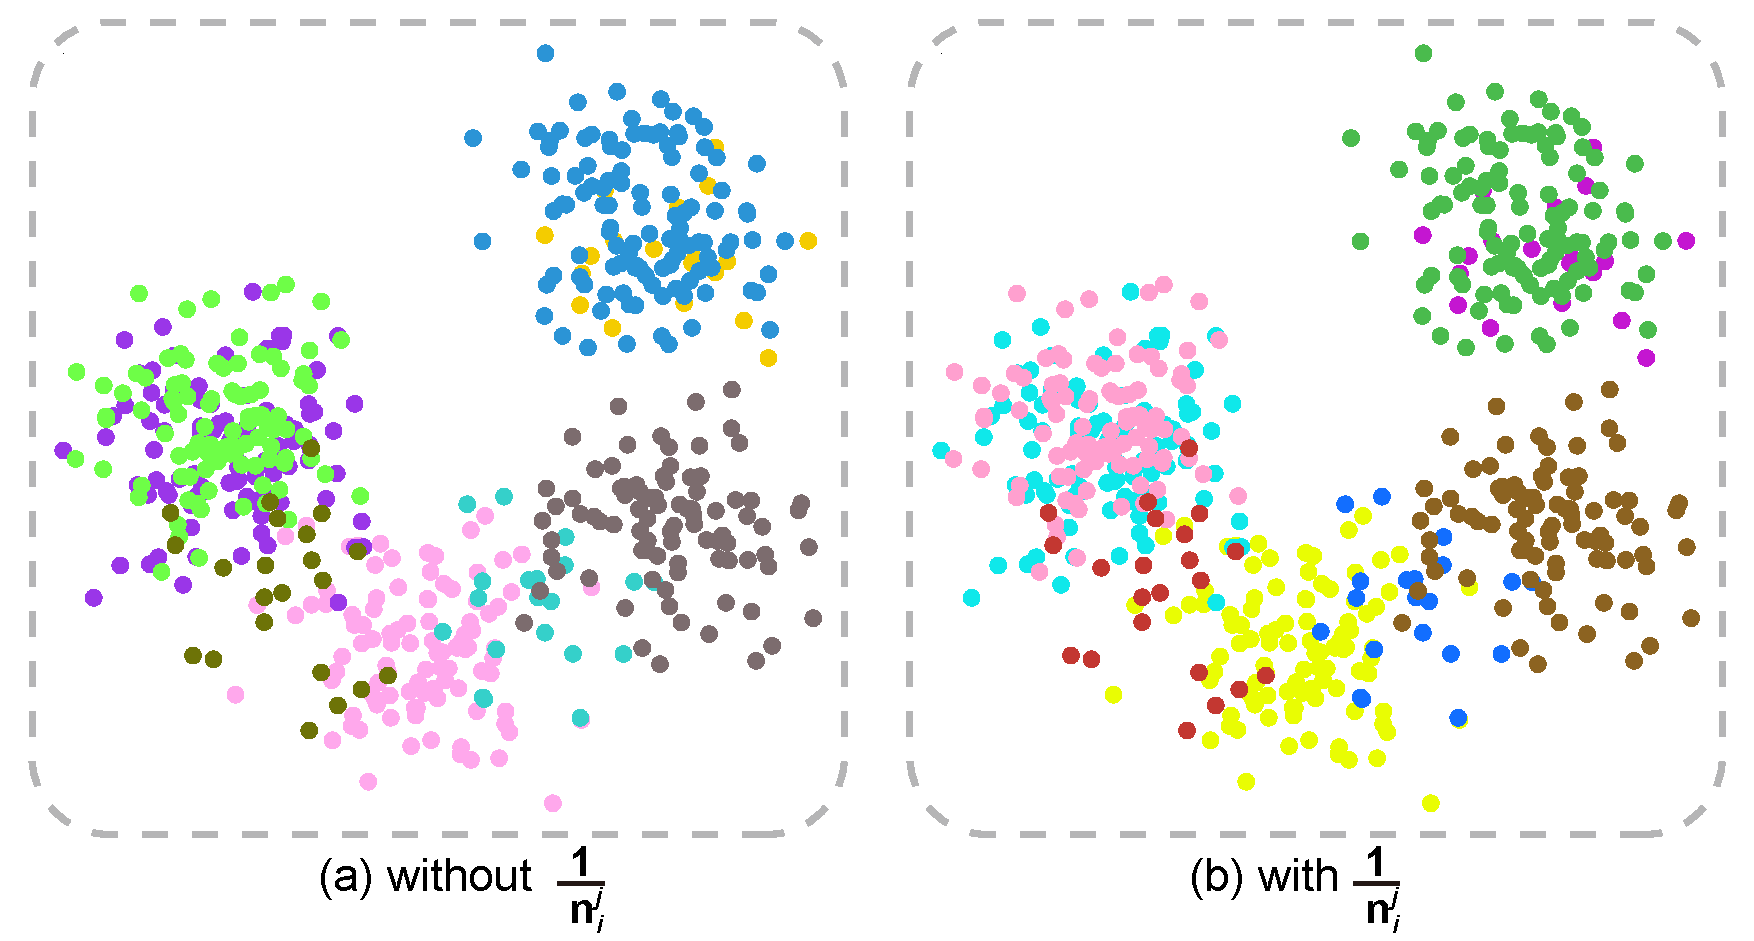
\includegraphics[width=0.8\textwidth]{figures/nij.pdf}
\caption{Effect of $\frac{1}{n^j_i}$: (a) without this term the small classes are hard to catch user's attention; (b) with this term, small classes are easy to find. Palettes are generated with same scatterplot.}
\vspace*{-3mm}
\label{fig:nij}
\end{figure}
%\vspace{.5em}

We can observe that when there's only one scatterplot and $\theta_i$ of each class is zero, then Equation.~\ref{eq:cosaliency} is very similar to the objective function of ~\cite{Wang2018}. Our method extends Wang et.al's work to multiple scatterplots with a carefully designed co-saliency model. Besides, we add $\frac{1}{n^j_i}$ to emphasize the class with less points. As shown in Fig.~\ref{fig:nij}(b), with this new term, the little classes, like red, blue and purple classes, become more discriminable.

%
\begin{figure}[ht]
\centering
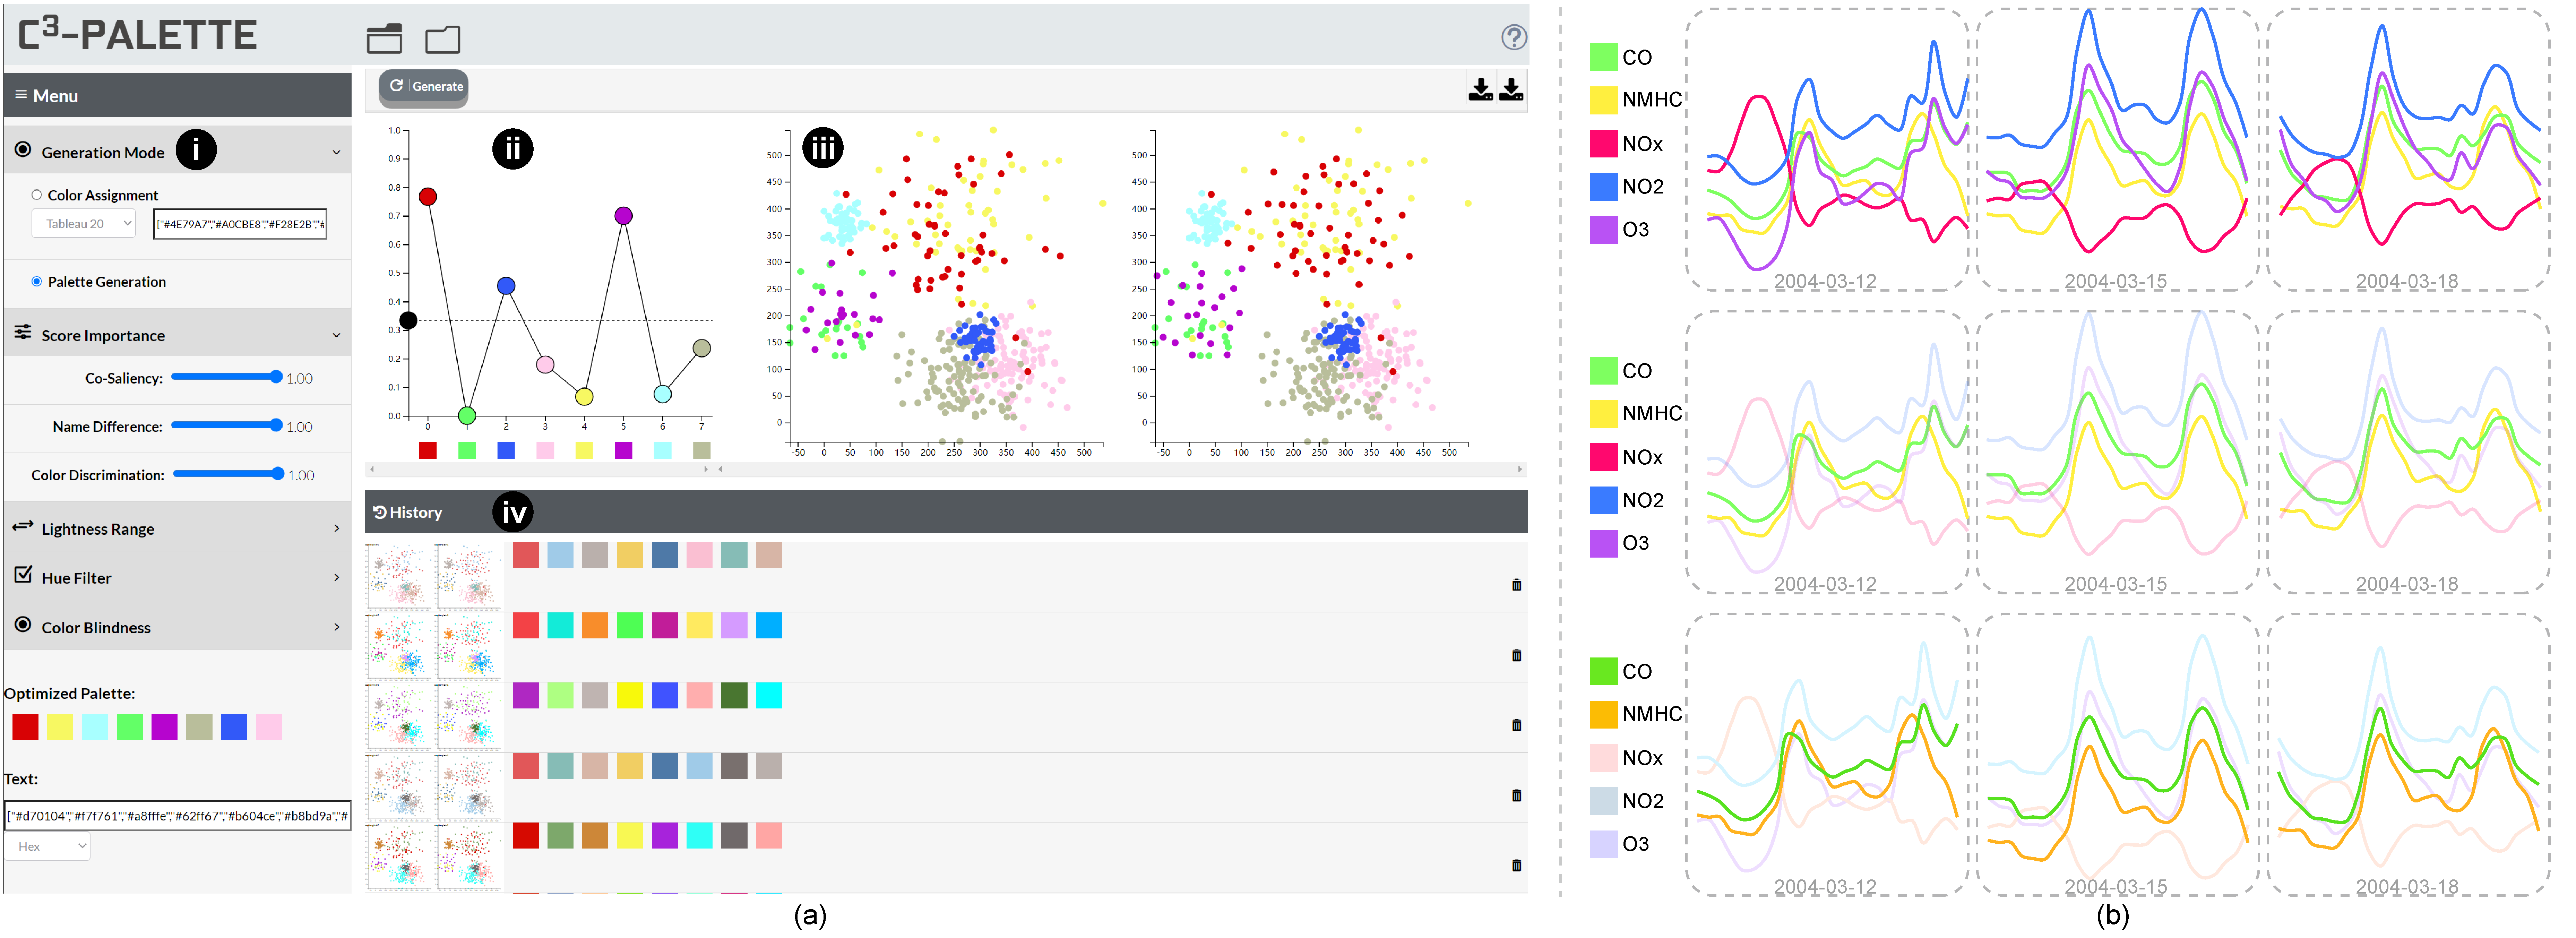
\includegraphics[width=0.8\columnwidth]{figures/interface-linechart.pdf}
\caption{(a) Screenshot of the interactive system consisted of four panels: (1) Settings Panel; (b Control Panel; (3) Visualization Panel; and (4) History Panel. (b)}
\vspace*{-3mm}
\label{fig:ui}
\end{figure}

\section{Interactive System}
\label{sec:interaction}
To help users interactively design colors for comparing multi-class scatterplots, we developed a web-based multi-view visualization tool \footnote{\small \url{https://c3-palette.github.io/}} (see Fig.~\ref{fig:ui}).
It consists of four coordinated views: (a) a settings panel, (b) a control panel for adjusting importance threshold $\kappa$ and even importance value of each class, (c) the juxtaposed visualizations, and (d) a history view. The control panel shows the decision which classes are highlighted, and the history view allows to quickly explore and access previous color mappings.

After uploading multiple categorical scatterplots, the user can either choose a default color palette or use our system to automatically generate color palettes. In this case, the system automatically finds an optimal color mapping scheme to colorize the input data, while each class is encoded as a circle where the x-axis represents class label and the y-axis indicates the importance of each class. By default, the importance is represented by the change degree and $\kappa$ is set to zero. User can drag the circle to modify the corresponding importance value. The $\kappa$ is controlled by a black circle on the y-axis which can also be dragged to modify. Our system finds a color mapping scheme to highlight the classes with large importance and renders the classes in ascending order of the corresponding importance. If users like the color mapping scheme, they can save it to the history view.

\vspace{1.5mm}
\noindent\textbf{Flexible Importance Manipulation}.
Using $\theta_i$  defined in Eq.~\ref{eq:cosaliency}, the classes whose importance values are larger than the threshold $\kappa$ will be highlighted.
Fig.~\ref{fig:ui}(b,c) show an example, where the three classes with the adjusted importance values larger than $\kappa$ are emphasized with salient \emph{red}, \emph{blue} and \emph{purple} colors, respectively.
This control panel allows users to select arbitrary classes of interest to highhlight by simply adjust circle position and $\kappa$ value. More use cases can be seen in Sec.~\ref{sec:caseStudy}.

\vspace{1.5mm}
\noindent\textbf{Color Vision Deficiency}.
To help people with a color vision deficiency, we allow users to generate palettes that can be used for different types of vision problem, such as protanomaly and deuteranomaly which result in poor red-green hue discrimination. This is achieved by adopting a color blindness simulator(the source code can be find at github: https://github.com/MaPePeR/jsColorblindSimulator) and then used our matrix for palette evaluation. Fig.~\ref{fig:blindness} show an example, where the left two images show the auto-generated results and the right are the simulated results perceived by people with protanomaly.

\begin{figure}[ht]
\centering
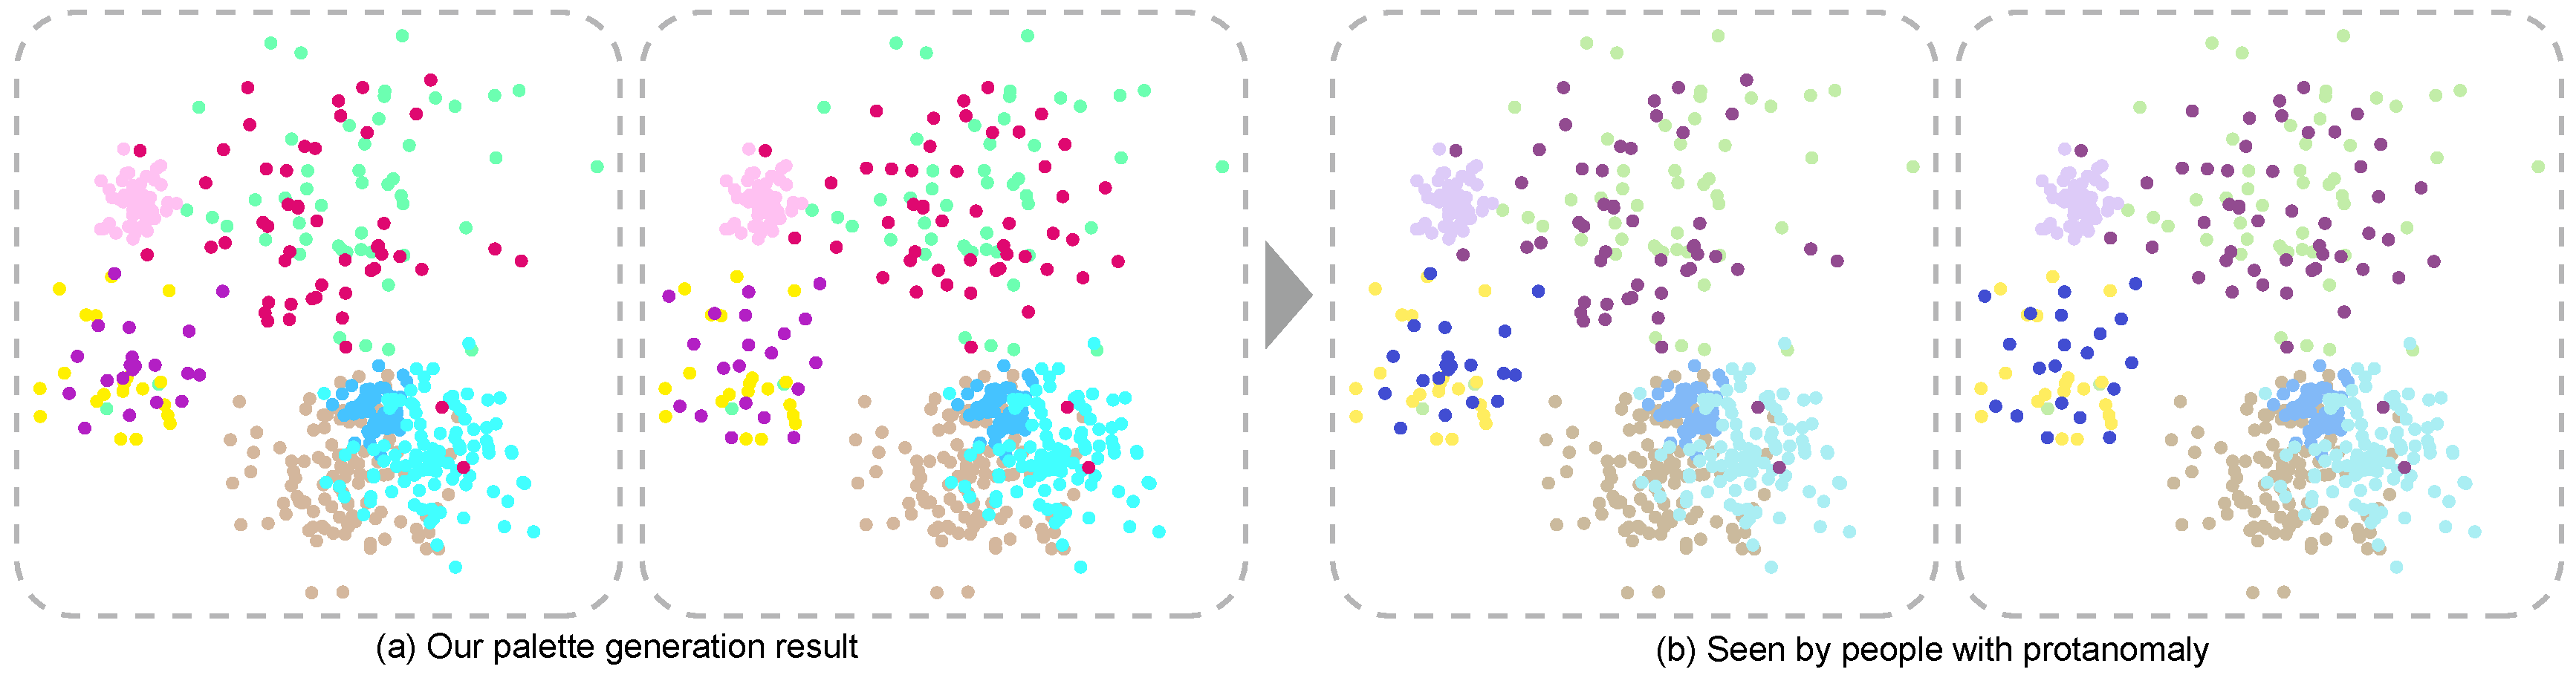
\includegraphics[width=0.96\linewidth]{figures/blindness.pdf}
\caption{Exploring the ability of our system to generate palettes for both people with normal vision and color blindness. (a) The automatic generated palette makes the two importance classes with large saliency while maintain good separability between other classes. (b) Simulated results for people with protanomaly. We can see our results maintain a good performance for color vision deficiency.}
\vspace*{-3mm}
\label{fig:blindness}
\end{figure}


\section {Evaluation}
\label{sec:results}

We evaluated the effectiveness of our method on supporting juxtaposed visual comparisons and the discriminability for reading scatterplots. % by applying it to scatterplots, as scatterplots are commonly used  for such comparisons.
We conducted two online controlled experiments through Amazon Mechanical Turk (AMT) with 217 participants in total, to evaluate how well our method can support people in \emph{observing changes} and \emph{visual separability} for multiple categorical scatterplots:
\begin{enumerate}
%\vspace{-3mm}
\item [(i)] \emph{Spotting the difference task}. To evaluate how well our method can support people in \emph{observing changes} for juxtaposed categorical scatterplots;
%\vspace{-3mm}
\item [(ii)] \emph{Counting class number task}. To evaluate whether our method can support the \emph{visual separability} of classes in each individual scatterplot, which is considered fundamental to juxtaposed comparison.
%%\vspace{-3mm}
%\item [(iii)] an eye tracking study to initially explore if our method helps people \emph{alleviate eye movement distance} when performing  juxtaposed comparison tasks.
%\vspace{-3mm}
%\item [(iv)] performing two case studies to show the usability of our methods for scatterplot matrix and time series data.
\end{enumerate}
%we use synthetic data for the first three studies while use real world data for the case study.

\vspace{.3em}
\noindent{\textbf{Independent Variables.}} In each of our studies, we investigated three independent variables: colorization method, change magnitude and change type.

\emph{Colorization method}: We used six different ways to colorize scatterplots, including four benchmark methods (\emph{Random Assignment}, \emph{Optimized Assignment}, \emph{Alpha Blending} and \emph{Palettailor}) and two experimental methods based on our approach (\emph{C3-Palette Assignment}, \emph{C3-Palette Generation}):
\begin{itemize}

     \item C1: \emph{Random Assignment} is randomly selecting and assigning colors from Tableau-20 palette to the classes.

     \item C2: \emph{Optimized Assignment} uses the optimized assignment approach~\cite{Wang2018} for one of the two scatterplots with an input of Tableau-20 color palette.

     \item C3: \emph{Alpha Blending} is achieved by setting the alpha of each unchanged class to $0.5$ while the changed classes remain to $1.0$ based on \emph{Optimized Assignment} result. We choose $0.5$ since the results also used in the discrimination task.
     \item C4: \emph{Palettailor} uses the method proposed by Lu et.al~\cite{Lu21} for single scatterplot palette generation. The palette is generated for one of the two scatterplots with the default settings.
     \item C5: \emph{C3-Palette Assignment} uses the color assignment optimization solution(Eq.~\ref{eq:cosaliency}) based on Tableau-20.
     \item C6: \emph{C3-Palette Generation} uses the unified color generation and assignment optimization method, and produced the results with the default settings($\omega_0=1.0$, $\omega_1=1.0$ and $\omega_2=1.0$).
\end{itemize}
Our approach are all using the default parameters $\lambda=0.4$ and $\kappa=0$.

\emph{Change magnitude} and \emph{Change type}: While the colorization method is the primary independent variable to be investigated, we are also interested in how the effect of different methods would vary based on the level of change between the two scatterplots and the different change type of classes. Thus we first define two types of changes that a class would have across multiple scatterplots: \emph{point number} and \emph{point position}. Then for each change type, we define three levels of change magnitude calculated using Eq.~\ref{eq:cm}: \emph{small}, \emph{medium}, and \emph{large}. (See the next paragraph for the detailed calculation.)

\vspace{.3em}
\noindent{\textbf{Scatterplot Dataset Generation.}}
The paired scatterplot datasets used in our studies were generated as follows.
First, we designed a set of multi-class scatterplots, each containing $8$ classes. Each class was generated using Gaussian random sampling and placed randomly in a $600 \times 600$ area.
Similar to~\cite{Lu21}, these classes belong to one of the four settings of varying size and density: small \& dense ($n=50, \sigma=20$), small \& sparse ($n=20, \sigma=50$),  large \& dense ($n=100, \sigma=50$), and large \& sparse (($n=50, \sigma=100$).

Then, for each scatterplot generated above, we produced its paired scatterplot by randomly choosing one or more classes and changing the positions or number of their data points.
%We focused on two common change types: \emph{point number} and \emph{point position}.
To systematically compute the changes, we defined two variables: \emph{change ratio} and \emph{number of changed classes}.
\emph{Change ratio} defines how large the change of a type is, ranging from 0 to 1; and {number of changed classes} defines the number of classes that are changed, ranging from 1 to 3 (to add
different levels of difficulty). We summarize our basic idea of data generation for each change type as below.
\begin{itemize}

     \item \emph{Point number}: For each class in the original scatterplot,  we calculated the new point number by multiplying the original number by ($1 \pm$ \emph{change ratio}). An addition means to increase the point number, which was implemented by generating the new points with the same distribution as the original class. Subtraction was achieved by randomly deleting data points from the original class.

     \item \emph{Point position}: Point position contains many types, such as class center position change and shape change. In our experiment, we use the two different position changes mentioned above. For center position change, the center of a class can be moved in a certain \emph{direction} with a specific \emph{distance}. We moved the center towards a random direction by a distance calculated by multiplying a maximal change distance ($400$ by default) by the \emph{change ratio}. For shape change, we define the shape of a class as the bounding box of its data points. We simulated a shape change of a class by modifying the density parameter of its Gaussian distribution to the opposite direction. For example, a small \& dense class ($n=50, \sigma=20$) would be changed into a small \& sparse ($n=50, \sigma=50$) class. In order to produce a new shape for a class, we first calculate the one-to-one mapping between the newly-generated class and the original class using ~\cite{kuhn1955hungarian} and then linearly interpolated the new point between each two points based on the \emph{change ratio} parameter. We randomly choose one change type when disturbing the class to be changed.
\end{itemize}
For each change type, we produced 300 candidate scatterplot pairs and then calculated the \emph{change magnitude} for each pair, and split all  pairs into three levels: \emph{small},  \emph{medium}, and \emph{large}.
Next, we randomly selected $2$ pairs from each change magnitude level for each change type and each number of changed classes. Thus in total we used $36$ paired scatterplot in each of the two studies. The detailed dataset is showed in Table.~\ref{tab:latinsquare}

\begin{table}[ht]
     \renewcommand\arraystretch{1}
     \centering
     \caption{Grouping of Datasets: $36$ datasets $\times$ $6$ conditions. C: condition; G: participant group; Position Small 1: point position change with small change magnitude for 1 changed class.}
     \label{tab:latinsquare}
     \begin{tabular}{lcccccccc}
     \hline
      & C1 & C2 & C3  & C4 & C5 & C6 \\

     \hline
     Dataset 1: Position Small 1 & \textbf{G1} & G2 & G3  & G4 & G5 & G6 \\
     Dataset 2: Position Small 1 & G6 & \textbf{G1} & G2 & G3  & G4 & G5 \\
     Dataset 3: Position Small 2 & G5  & G6 & \textbf{G1} & G2 & G3 & G4 \\
     Dataset 4: Position Small 2 & G4 & G5  & G6 & \textbf{G1} & G2 & G3 \\
     Dataset 5: Position Small 3 & G3 & G4 & G5  & G6 & \textbf{G1} & G2 \\
     Dataset 6: Position Small 3 & G2 & G3 & G4  & G5 & G6 & \textbf{G1} \\
     Dataset 7: Position Medium 1 & \textbf{G1} & G2 & G3  & G4 & G5 & G6 \\
     Dataset 8: Position Medium 1 & G6 & \textbf{G1} & G2 & G3  & G4 & G5 \\
     ... & & & & & & &\\
     Dataset 35: Number Large 3 & G3 & G4 & G5  & G6 & \textbf{G1} & G2 \\
     Dataset 36: Number Large 3 & G2 & G3  & G4 & G5 & G6 & \textbf{G1}  \\

     \hline
     \end{tabular}
     \end{table}
%
%\subsection{Numeric Study}
%\label{subsec:quantitystudy}
%To evaluate whether our approach can fundamentally support the visual separability of the classes in each scatterplot, we conducted a numeric study using the \emph{class visibility metric} proposed by Kim et al.~\cite{lee2013perceptually}. We calculated each scatterplot in every pair, and used the average value as the final score of the pair. We then compared the scores across different colorization methods.
%
%%\vspace{.3em}
%%\noindent{\textbf{Results.}}
%
%\begin{figure}[h]
%\centering
%\includegraphics[width=0.9\linewidth]{figures/classVisibility.pdf}
%\caption{Average class visibility score of the 36 synthetic scatterplot pairs of each color mapping scheme.}
%\vspace*{-3mm}
%\label{fig:classVisibility}
%\end{figure}
%
%As shown in Fig.~\ref{fig:classVisibility}, \emph{Ours Generation} has the highest score on average. \emph{Ours Tableau-10} is sometimes higher than \emph{Random Tableau-10}. The two conditions based on the Tableau-20 palette have the lowest scores, and \emph{Ours Tableau-20} appears to be slightly lower than \emph{Random Tableau-20}. This might be caused by the palette used in these conditions. Since Tableau-20 consists of both saturated and de-saturated colors, \emph{Ours Tableau-20} tends to select several de-saturated colors for the classes that change less in order to make strongly changed classes more salient. Yet that might diminish the visual separability of the classes.

\subsection{Experiment 1: Spotting the Difference}
\label{subsec:onlinestudy1}

To evaluate how well our approach can assist observing changes between juxtaposed categorical scatterplots, we conduct an online ``spot-the-difference'' experiment through Amazon Mechanical Turk (AMT) with 136 participants.
%We show participants a set of paired multi-class scatterplots, and ask them to find a known number of classes that have been changed within $60$ seconds.  Error rate and consuming time are recorded for analysis.

\vspace{.3em}
\noindent{\textbf{Hypotheses.}} We hypothesized that our approach would generally be more effective than the benchmark methods on the juxtaposed comparison tasks, and that this effect would vary based on \emph{change magnitude} or \emph{change type}.
%In this experiment, our major goal is to investigate if our co-saliency based color design formulation would affect the performance of observing changes between multiple datasets.
\begin{itemize}[noitemsep]
\setlength{\itemsep}{5pt}
    \item[\textbf{H1.}] Our color generation method (\emph{C3-Palette Generation}) outperforms the benchmark conditions (\emph{Random Assignment}, \emph{Optimized Assignment}, \emph{Alpha Blending} and \emph{Palettailor}) on the task performance.

    \item [\textbf{H2.}] Our color assignment method (\emph{C3-Palette Assignment}) using a color palette with a large range of brightness and saturation (\emph{Tableau-20}) outperforms the benchmark conditions (\emph{Random Assignment}, \emph{Optimized Assignment}, \emph{Alpha Blending} and \emph{Palettailor}) on the task performance.

    \item [\textbf{H3.}] Other independent variables(\emph{change type} and \emph{change magnitude}) would also affect user performance on the task performance.

    \item [\textbf{H4.}] There would be an interaction effect between colorization methods and other independent variables(\emph{change type} and \emph{change magnitude}). Specifically, the difference between the effect of our methods (\emph{C3-Palette Generation} and \emph{C3-Palette Assignment}) and that of the benchmark methods (\emph{Random Assignment}, \emph{Optimized Assignment}, \emph{Alpha Blending} and \emph{Palettailor}) would change based on the different variable.
\end{itemize}

% For content we can refer to:
% \url{http://www.yunhaiwang.net/infoVis2020/palettailor/pdf/vis20a-sub1326-i6.pdf}
% \begin{itemize}
%     \item List the assignment methods: ours and the benchmarks.
%     \item Recap the definition of \emph{change magnitude} and \emph{change type}.
% \end{itemize}

\subsubsection{Experimental Design}
%In this experiment, each participant completed a ``spot-the-difference'' task that contains $40$ paired multi-class scatterplots.
%To colorize the paired scatterplots, we adopt the five visualization methods -- three of them are optimized or generated based on our approach (\emph{Ours Tableau-10}, \emph{Ours Tableau-20} and \emph{Ours Generation}), while the other two are random ones  (\emph{Random Tableau-10} and \emph{Random Tableau-20}).
\
\newline
\vspace{.3em}
\noindent{\textbf{Task \& Measures.}}
In this experiment, each participant was asked to perform a \emph{spot-the-difference} task. Inspired by the Spot the Difference game where one needs to compare a pair of similar pictures to detect their differences~\cite{Fukuba2009}, we asked participants to identify all the classes that have been changed in two scatterplots. At the beginning of each trial, the number of changed classes was provided. Each participant was asked to select all the changed classes by clicking the points belonging to these classes in either of the scatterplots.

For each participant, we measured the \emph{time} taken for each trial, and counted the errors ($0/1$) indicating whether the actual changed classes are aligned with the participant's response. Note that if any of the changed classes was mistakenly identified, the trial would be considered as ``wrong'' (1).

While the participant was instructed to do the task ``\emph{as accurately as possible}'', we set a $60$-second time limit for each trial for fear that user might spend too much time on the trial. If the participant could not find all the changed classes during the time limit, they were directed to the next trial. There also will appear a ``\emph{Can't Find it}'' button after $30$ seconds.
This was done since we observed from the pilot study that when participants spent too much time on a single trial, they may decide to quit by selecting a class randomly(which will lead to an incorrect answer) or to spend more time till they get the correct answer or the time limit (which will lead to increasing time spent on the trial). This subject decision would add noise to our measurements. Thus we added a $30$-second time limit, which was informed by our pilot study, where over $85\%$ correct trials were completed within $30$ seconds.

\vspace{.3em}
\noindent{\textbf{Experiment Organization.}} We tested the effects of the $6$ method conditions across $36$ paired multi-class scatterplot datasets using a \emph{between-subject} experiment design. To avoid ordering effects, where the participant would get familiar with a dataset after seeing it several times, each participant was assigned to a group and saw a specific subset of datasets under different conditions. We used a Latin Square grouping (see Table.~\ref{tab:latinsquare}) to organize the trials for each participant. %$Thus, there were $6$ participant groups and each of them had $40$ trials in total. See the supplementary material for more details.

In addition, some participants might apply a ``shortcut'' strategy when seeing a class that is obviously more salient than the others, especially under the \emph{C3-Palette Assignment} and \emph{C3-Palette Generation} conditions. Thus, for quality control, we added $4$ sentinels which were very simple trials with only one changed class and a large change magnitude, and we assigned a de-saturated color to the changed class that made it less salient. We add these 4 distractor trials to each group to identify whether the participants is doing the task seriously and reject the results with more than two wrong trials.
%especially to avoid preferences of \emph{Our Generation} method.
%Only answers with a over $50\%$ accuracy were accepted.

Finally, there were $6$ participant groups and each of them had $40$ trials in total. To further avoid learning effects between trials, we randomly shuffled the display orders of all scatterplot pairs, and randomly placed the two scatterplots in each pair on the left or right side.

\begin{table}[ht]
\renewcommand\arraystretch{1}
\centering
\caption{Participants details for each task.}
\label{tab:participantDetail}
\begin{tabular}{|c|c|c|c|c|}
\hline
\multirow{2}{*}{\textbf{Task \& Group}} & \multicolumn{2}{c|}{Spotting the Difference} & \multicolumn{2}{c|}{Counting class number} \\
\cline{2-5}
& Pilot(28) & Formal(108) & Pilot(29) & formal(52) \\
\hline
Group 1 & 5 & 18 & 5  & 9 \\
\hline
Group 2 & 5 & 17 & 5  & 8 \\
\hline
Group 3 & 5 & 19 & 4  & 8 \\
\hline
Group 4 & 3 & 17 & 5  & 9 \\
\hline
Group 5 & 5 & 19 & 5  & 9 \\
\hline
Group 6 & 5 & 18 & 5  & 9 \\
\hline
\end{tabular}
\end{table}

\begin{figure*}[t]
\centering
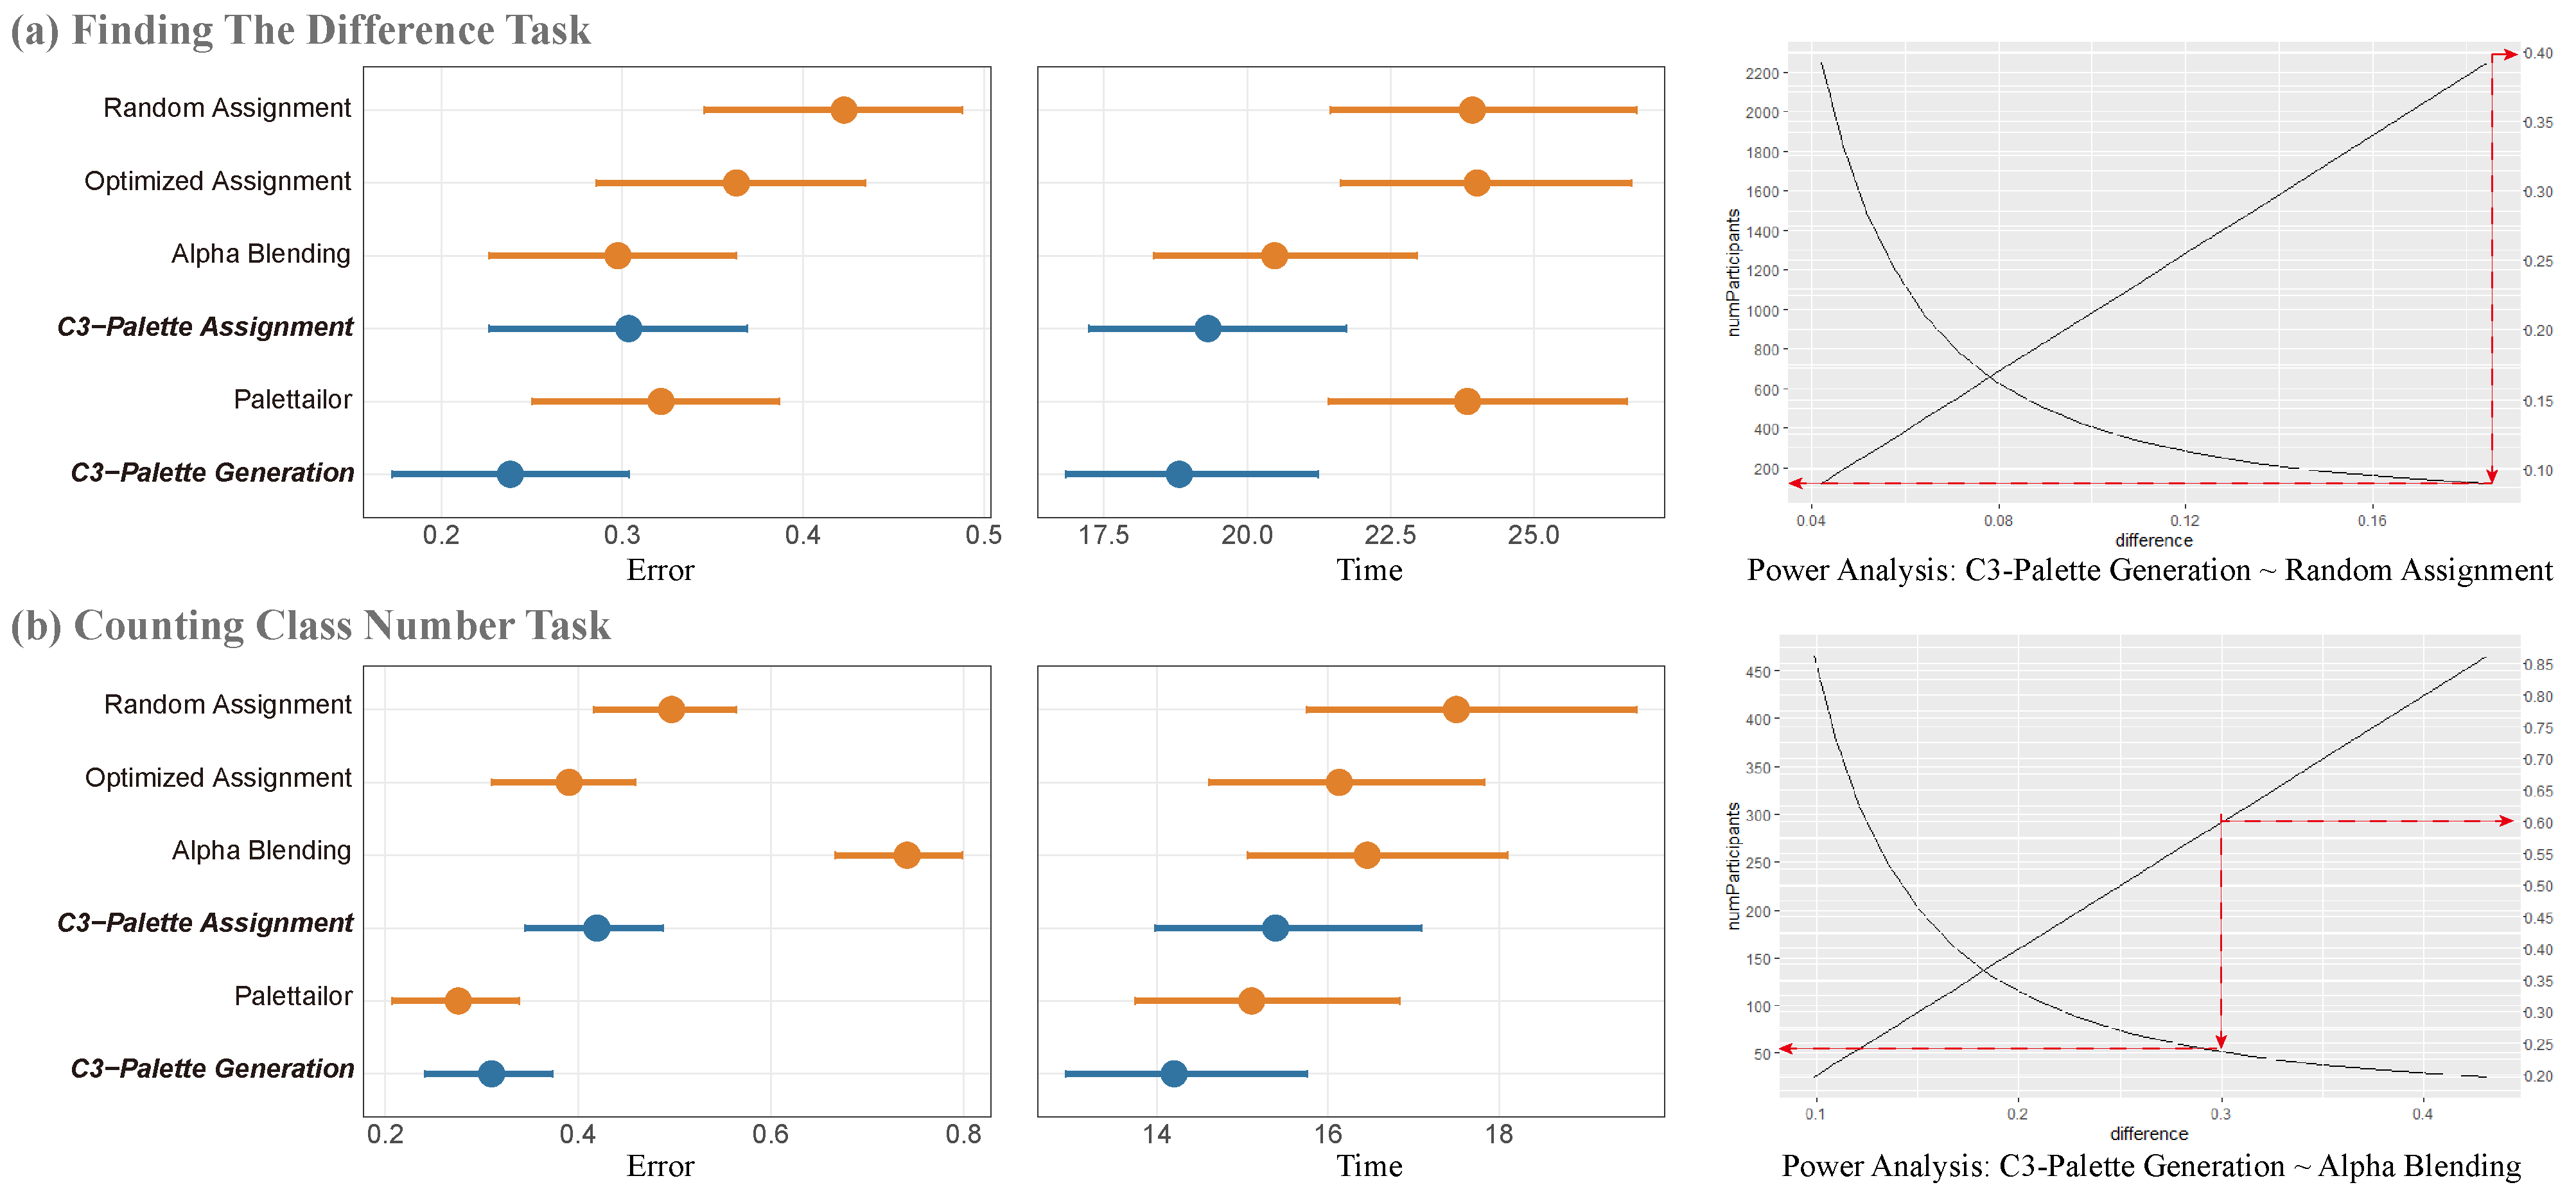
\includegraphics[width=1\linewidth]{figures/user-result-pilot.pdf}
\caption{Confidence interval plots and power analysis for the two pilot studies.
}
\vspace*{-3mm}
\label{fig:pilotResults}
\end{figure*}

\vspace{.3em}
\noindent{\textbf{Pilot Study \& Power Analysis.}}
We conducted a pilot study involving 28 participants to check the experimental setup and determine the parameters, such as the time limit for a trial. The results are shown in Fig.~\ref{fig:pilotResults}(a).
Harnessing by the pilot study, we also obtained our expected effect sizes, which were in further fed into a power analysis. With an effect size Cohen's $d$ of $0.4$, alpha level of $0.05$ and beta level of $0.8$, the power analysis suggested a minimum number of $100$ participants for the spot-the-difference task. %See the supplementary material for more details.


\vspace{.3em}
\noindent{\textbf{Participants.}}
We recruited $108$ participants(as shown in Table.~\ref{tab:participantDetail}) for the experiment on Amazon Mechanical Turk.
According to the completion time in the pilot study, we paid each participant \$$1.5$ for the task based on the US minimum hourly wage.
No participant claimed color vision deficiency on their informed consent.

\vspace{.3em}
\noindent{\textbf{Procedure.}}
Each participant went through the following steps in our experiment: (i) viewing a user guide of the task and completing three training trials; (ii) completing each trial as accurately as possible; (iii) providing demographic information.

\begin{figure*}[t]
\centering
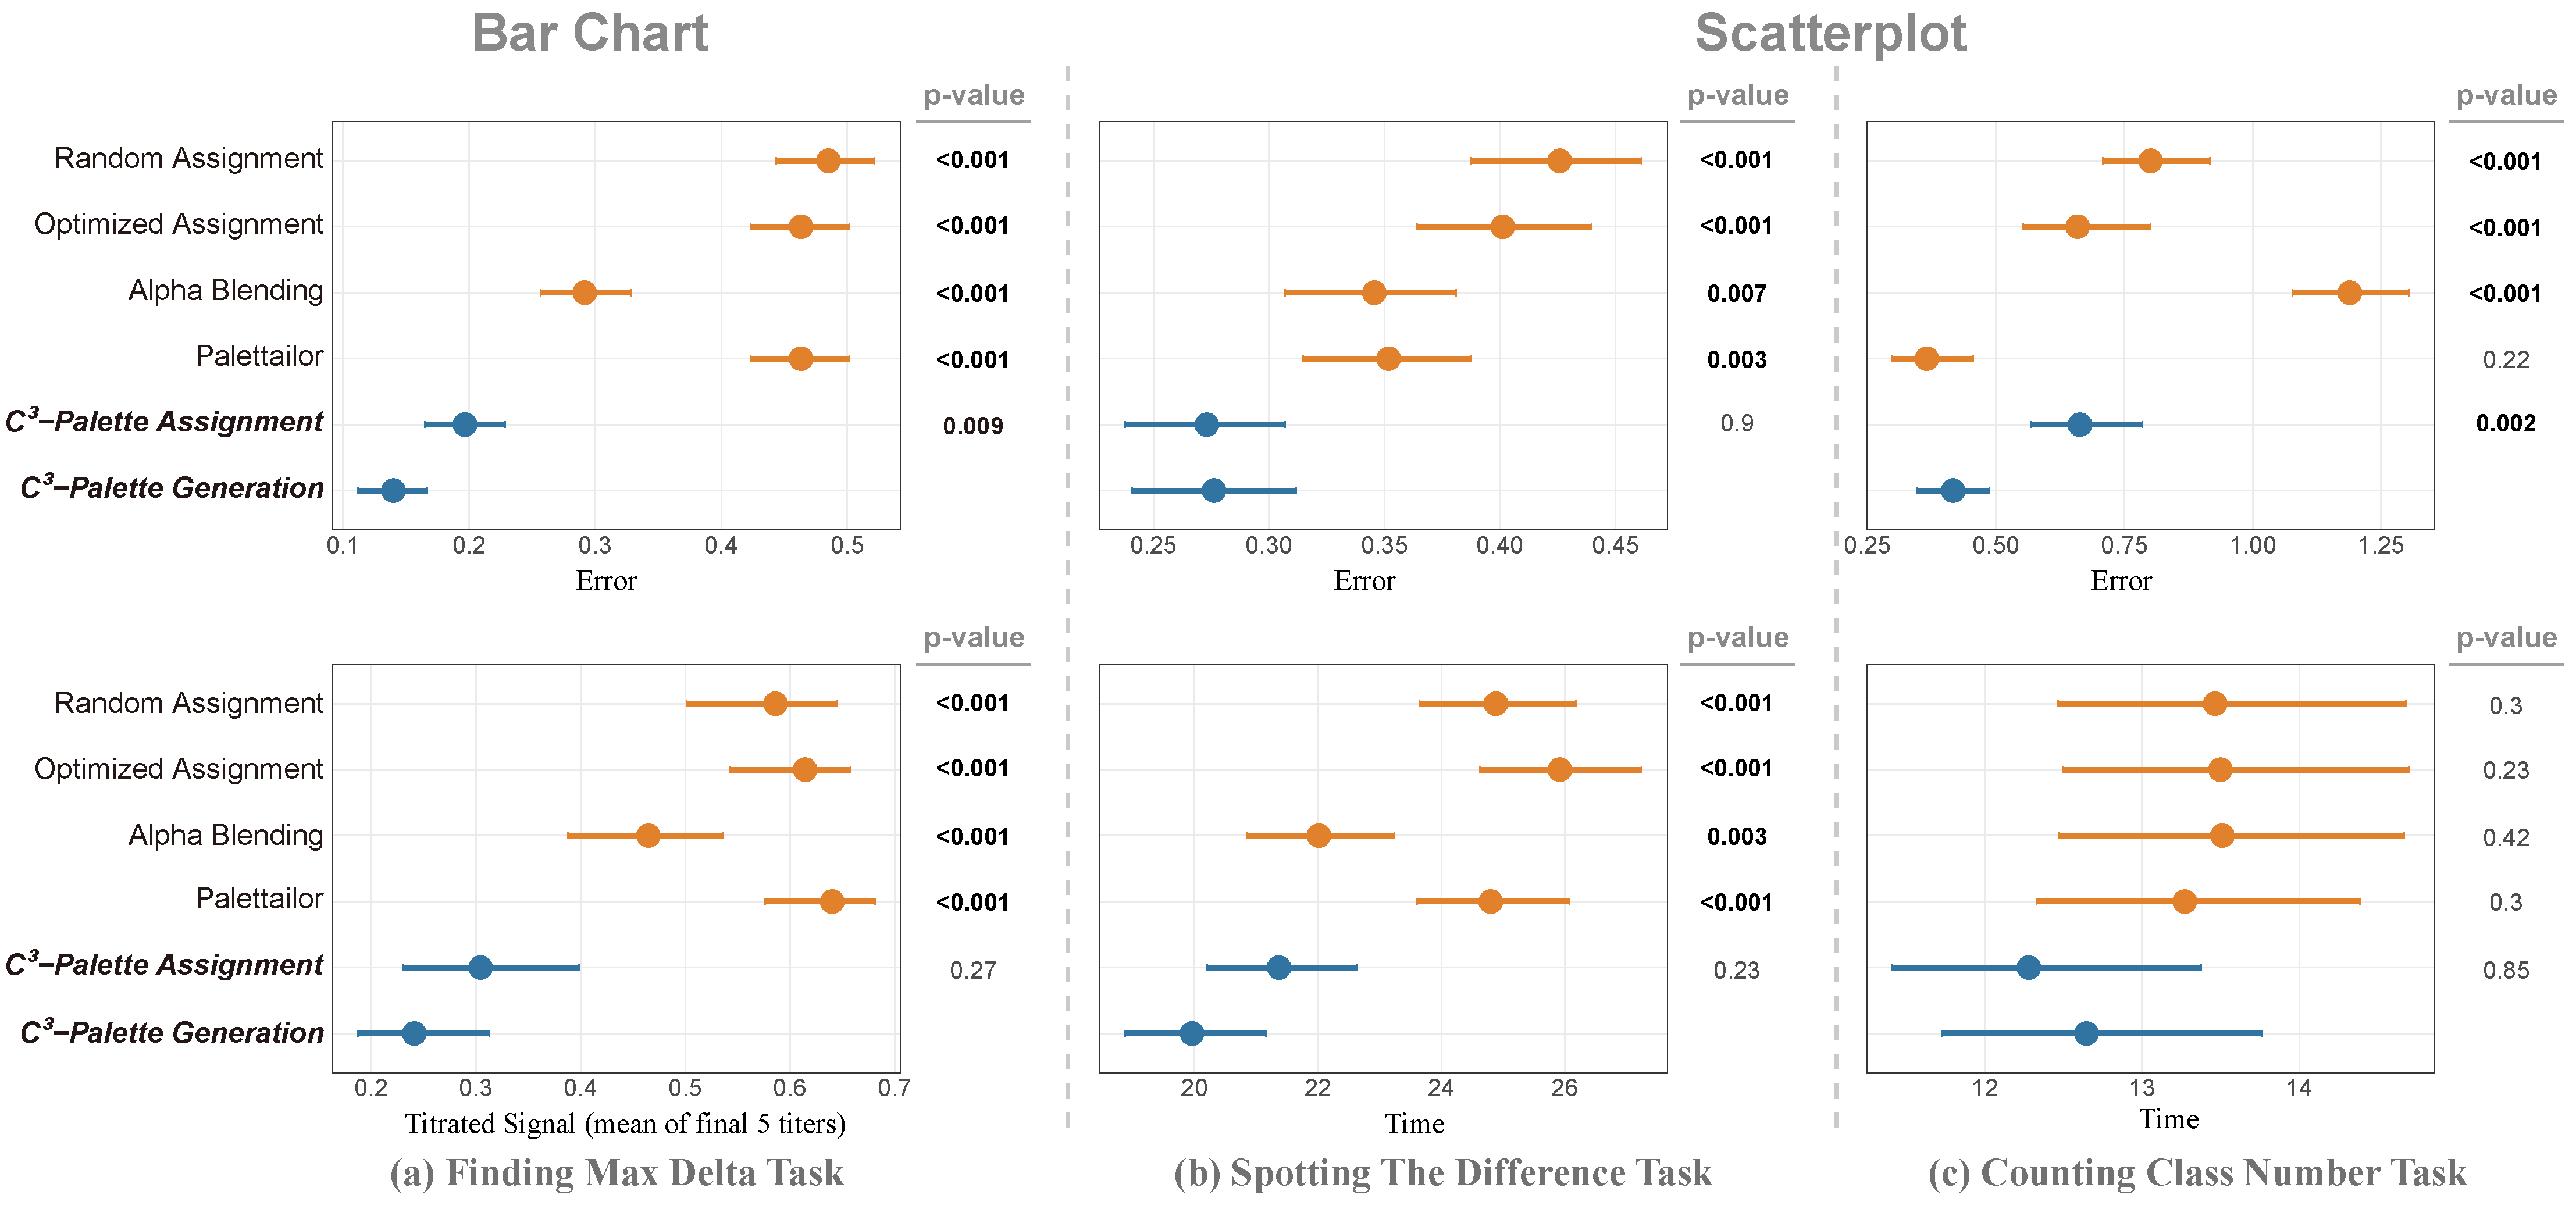
\includegraphics[width=1\linewidth]{figures/user-result-formal.pdf}
\caption{Confidence interval plots and statistical tables for the two online controlled experiments. Error bars represent $95\%$ confidence intervals. Each table shows the statistical test results of C3-Palette Generation condition with other conditions, including the mean with $95\%$ confidence interval ($\mu\sim$95\%CI), the W-value and p-value from the Mann-Whitney test, and the effect size ($d\sim$95\%CI).
}
\vspace*{-3mm}
\label{fig:userResults}
\end{figure*}

\subsubsection{Results}
\
\newline
Following previous studies, we analyzed the results using 95\% confidence intervals, and also conducted Mann-Whitney tests to compare the differences between conditions. The non-parametric test was used due to observations of non-normally distributed data from our pilot study. In addition, we computed the effect size using \emph{Cohen's d}, i.e., the difference in means of the conditions divided by the pooled standard deviation. We used ANOVA to examine the interaction effect between variables.


Results of the online experiment are shown in Fig.\ref{fig:userResults} (a).
First, we found that our approach(\emph{C3-Palette Assignment} and \emph{C3-Palette Generation}) leads to a significantly lower error rate than all benchmark conditions. For consuming time, \emph{C3-Palette Generation} has significantly less time (\emph{$p = 0.003$}) than \emph{Alpha Blending} condition while \emph{C3-Palette Assignment} has no significant difference (\emph{$p = 0.095$}), and our approach has significantly less time than all other benchmark conditions(\emph{$p < 0.001$}). The result indicates that our palette generation method(\emph{C3-Palette Generation}) has a better performance than benchmark conditions in the ``spot-the-difference'' task (\textbf{H1} confirmed). As for color palette with a larger range of brightness and saturation, our approach(\emph{C3-Palette Assignment}) is better than most conditions and is at least comparable to \emph{Alpha Blending} condition(\textbf{H2} confirmed).


%Second, we compared our approach to other conditions based on two different change types(\emph{Point Number Change} and \emph{Point Position Change}).
%For \emph{Point Number Change}, as shown in the top row of  Fig.\ref{fig:userResults} (c), our approach(\emph{C3-Palette Assignment} and \emph{C3-Palette Generation}) leads to a significantly lower error rate than all benchmark conditions, including \emph{Random Assignment} and \emph{Optimized Assignment}(\emph{$p < 0.001$}), \emph{Alpha Blending} and \emph{Palettailor}(\emph{$p < 0.05$}). \emph{C3-Palette Generation} condition has a better performance on consuming time than all other benchmark conditions, while \emph{C3-Palette Assignment} is just comparable to \emph{Alpha Blending} condition.
%For \emph{Point Position Change}, we observed that our approach has significant lower error rate than \emph{Random Assignment} and \emph{Optimized Assignment}(\emph{$p < 0.01$}), while there's no significant difference with \emph{Alpha Blending} and \emph{Palettailor}. \emph{C3-Palette Generation}) leads to a significantly lower consuming time than all benchmark conditions(\emph{$p < 0.001$}) except \emph{Alpha Blending}(\emph{$p = 0.044$})(\textbf{H3} confirmed).
Second, we compared error and time with regard to different change magnitudes, and found that smaller magnitude leads to larger error rate and consuming time (as shown in Fig.\ref{fig:userResultsVar} (a) left). This indicates that there exists an significant interaction effect between \emph{change magnitude} and performance, i.e., \emph{change magnitude} would affect user performance. We did the same test to \emph{change type}, the results show that \emph{point number change} is much more difficult than \emph{point position change}(\textbf{H3} confirmed).


Finally, we did not find significant interaction effect between \emph{colorization methods} and \emph{change magnitude} or \emph{change type}, meaning that the effect of our method is not necessarily influenced by the magnitude of change between the two scatterplots or the different change type of classes (\textbf{H4} not confirmed).

\begin{figure*}[h]
\centering
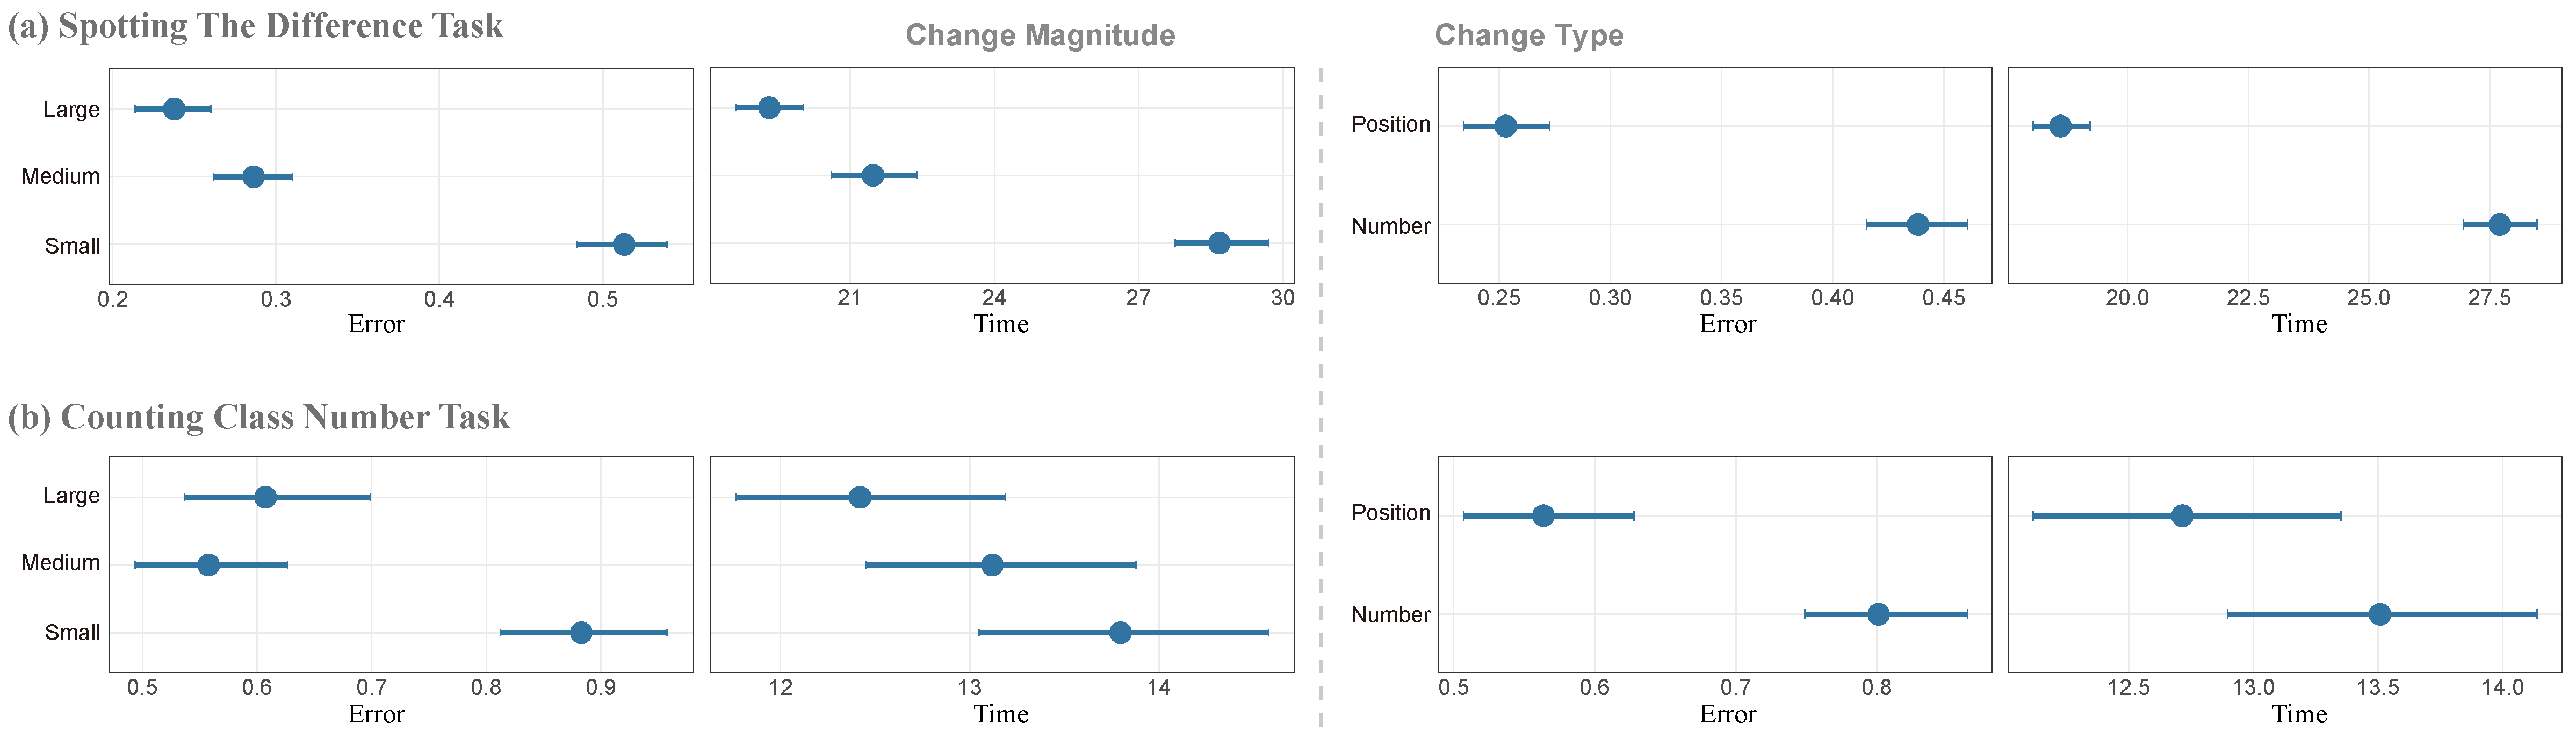
\includegraphics[width=1\linewidth]{figures/user-result-formal-variables.pdf}
\caption{Confidence interval plots for the two online controlled experiments. (left) Plots for \emph{change magnitude} based on error and time; (right) plots for \emph{change type} based on error and time.
}
\vspace*{-3mm}
\label{fig:userResultsVar}
\end{figure*}

\subsection{Experiment 2: Counting Class Number}
\label{subsec:onlinestudy2}
To evaluate whether our approach can fundamentally support the visual separability of the classes in each scatterplot, we conduct an online ``counting class number'' experiment through Amazon Mechanical Turk (AMT) with 81 participants. The experimental design was similar to the first study, but we set up with different task during the experiment.
We expected to see different patterns of the discriminability across different conditions. Specifically, our methods would lead to a shorter error and time than \emph{Random Assignment} and \emph{Alpha Blending} conditions.

\vspace{.3em}
\noindent{\textbf{Hypotheses.}} We hypothesized that our approach would generally be more effective than the benchmark methods on the discrimination tasks, and that this effect would not vary based on \emph{change magnitude} or \emph{change type}.
\begin{itemize}[noitemsep]
\setlength{\itemsep}{5pt}
    \item[\textbf{H1.}] Our color generation method (\emph{C3-Palette Generation}) outperforms the benchmark conditions (\emph{Random Assignment}, \emph{Optimized Assignment}, \emph{Alpha Blending}) and our assignment method(\emph{C3-Palette Assignment}), while is comparable to  \emph{Palettailor} on the task performance.

    \item [\textbf{H2.}] Our color assignment method (\emph{C3-Palette Assignment}) based on \emph{Tableau-20} outperforms the benchmark conditions (\emph{Random Assignment}, \emph{Alpha Blending}), while is comparable to \emph{Optimized Assignment} condition on the task performance.

    \item [\textbf{H3.}] Other independent variables(\emph{change magnitude} and \emph{change type}) would have no effect on discrimination task between different conditions.

    \item [\textbf{H4.}] There would be no interaction effect between colorization methods and other independent variables(\emph{change type} and \emph{change magnitude}).
\end{itemize}
\subsubsection{Experimental Design}
\
\newline
\vspace{.3em}
\noindent{\textbf{Task \& Measures. }}
Following previous methodologies~\cite{Wang2018, Lu21}, each participant was asked to perform a \emph{counting class number} task.  We asked participants to identify how many classes(colors) are there in the given two scatterplots and then choose an answer among several options below the two scatterplots. We recorded the participant's answer and response time for each trial, and counted the \emph{error}  by calculating the differences between the participant's answer and the actual number of classes(each scatterplot has $8$ classes in our experiment). %is $1$ if the participant's response not equal to the actual class number, else $0$.


\vspace{.3em}
\noindent{\textbf{Pilot Study \& Power Analysis.}}
This setting is similar to Experiment 1. We invited $29$ participants to do the pilot study and the results were in further fed into a power analysis. With an effect size Cohen's $d$ of $0.6$, the power analysis suggested a minimum number of $50$ participants for the discriminability task. See the supplementary material for more details.

\vspace{.3em}
\noindent{\textbf{Participants.}}
We finally recruited $52$ participants(as shown in Table.~\ref{tab:participantDetail}) for the experiment on Amazon Mechanical Turk.
According to the completion time in the pilot study, we paid each participant \$$1.5$ for the task based on the US minimum hourly wage.
No participant claimed color vision deficiency on their informed consent.

\subsubsection{Results}
\
\newline
Results of this visual separability experiment are shown in Fig.\ref{fig:userResults} (b).
Through this study we found that first \emph{C3-Palette Generation} is comparable to \emph{Palettailor} while leads to a significantly lower error rate(\emph{$p<=0.001$}) than all other benchmark conditions. Specifically, \emph{C3-Palette Generation} has a significantly lower error rate(\emph{$p=0.002$}) than \emph{C3-Palette Assignment}(\textbf{H1} confirmed).
Second, \emph{C3-Palette Assignment} has higher performance than the benchmark conditions (\emph{Random Assignment}, \emph{Alpha Blending}) and is comparable to \emph{Optimized Assignment}(\textbf{H2} confirmed).
For other independent variables, as shown in Fig.\ref{fig:userResultsVar} (b), we found that there existed a significant difference between \emph{Small change magnitude} and \emph{Medium} and \emph{Large}. \emph{Point position change} has a much lower error rate than \emph{point number change}. And their time has both a tendency to gradually increase. This indicates that \emph{change magnitude} and \emph{change type} might have an effect on discrimination task between different conditions (\textbf{H3} not confirmed).
Finally, we did not find significant interaction effect between \emph{colorization methods} and \emph{change magnitude} or \emph{change type}, meaning that the effect of different methods for visual discriminability is not
necessarily influenced by the magnitude of change between the two scatterplots or the different change type of classes (\textbf{H4} confirmed).
\vspace{.3em}
\subsection{Discussion}
In summary, we evaluated the effectiveness of our approach against the benchmark conditions through two online studies.
We found that first, our methods outperform the benchmark methods on juxtaposed comparison tasks, and their effects are not necessarily influenced by the change magnitude of the two scatterplots or the change type of each class.
The performance of \emph{Optimized Assignment} is comparable to \emph{Random Assignment}, this is reasonable, since \emph{Optimized Assignment} mainly cares about the visual separability of different classes, thus it might assign the less salient color to the changed class while \emph{Random Assignment} would assign salient color even though the whole separability of the scatterplot is not very good. This also provides an explanation for \emph{Alpha Blending} which is based on the result of \emph{Optimized Assignment}.
Second, our experimental methods (\emph{C3-Palette Generation} and \emph{C3-Palette Assignment}) generally support the fundamental visual separability of the classes. It is worth noting that the error rate of \emph{C3-Palette Generation} is comparable to \emph{Palettailor} which is the start-of-the-art palette generation method for visual discriminability, while \emph{C3-Palette Assignment} is comparable to \emph{Optimized Assignment} which is the start-of-the-art palette assignment method for visual discriminability. This indicates that our approach maintains the class distinction of the scatterplot while enhances the class saliency to help observe changes between different scatterplots.
Third, we found that \emph{change magnitude} and \emph{change type} influence the performance of the \emph{counting class number} task. The potential explanation is that large change between scatterplots will attract participants' attention, thus make it easy to distinct different classes. This is also reasonable for \emph{change type} since point position change is easier to distinguish than point number change.
It's obvious that \emph{Alpha Blending} has a much lower error rate than other methods for discrimination task. As one of the participants said, ``The ones that were harder were ones that had colors that when they overlapped would change color. It made it hard to tell if it was the same color or if it was a new color. When the colors were uniform and all the same opacity, it was much easier.'' \emph{Alpha Blending} condition changes the opacity of unchanged classes to make the unchanged classes more distinct, but this will generate new color from color blending, so as to make it hard to distinct colors.

Some limitations exist in our evaluation.
First, our experiment mainly focuses on error rate and time comsuming, while other measurements are not explored, such as click order of the changed classes and time consuming for each click. These might reflect some interesting results for different \emph{cluster type}.
Second, our experiment focuses on identifying the differences between two scatterplots, which is a simplified situation, since in real-world cases often more than two visualizations are compared.
Third, we cannot further analyze the effect of \emph{change type}, given the current study design, though we did observe some trends that for certain types of change, our methods are more effective.
That brings us to a series of more fundamental questions: how can we properly define the types of changes? What is the just noticeable change magnitude for each change type?
Further research is needed to answer these questions so that our approach can be thoroughly evaluated.

\section{Interactive System}


\begin{figure}[ht]
\centering
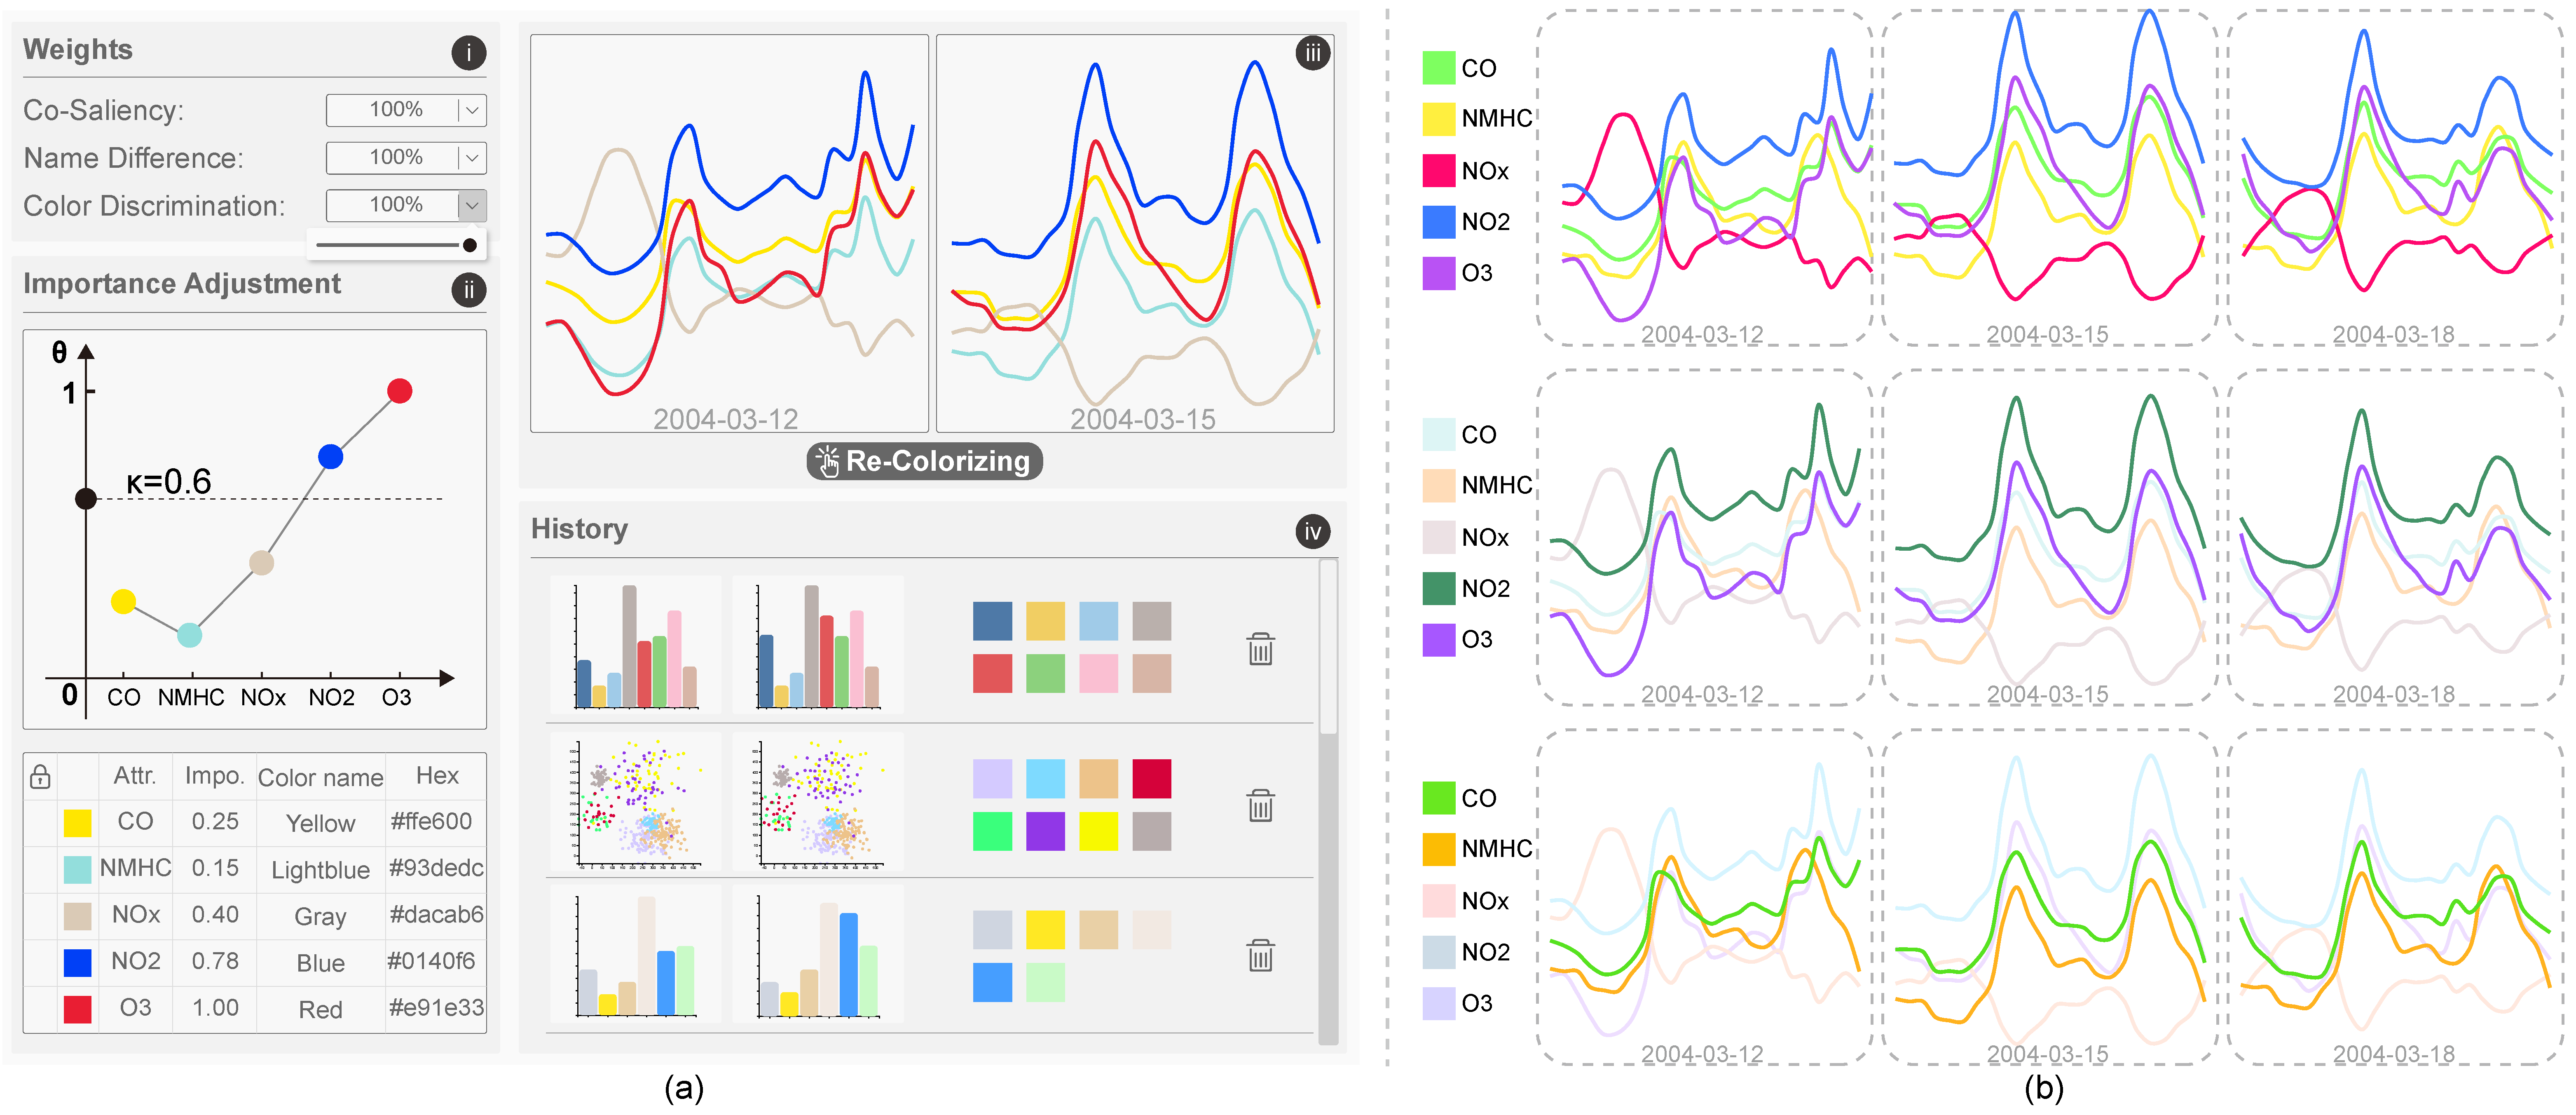
\includegraphics[width=1.0\columnwidth]{figures/interface.pdf}
\caption{Our interactive colorization system and a case study. (a) Screenshot of the interactive system consisted of four panels: (i) control panel; (ii) importance adjustment panel; (iii) visualization panel; and (iv) history panel. (b) Using this system to explore the changes of gases in an air quality data set~\cite{DEVITO2008750}: (top) The automatic generated palette creates salient colors for  lines; (middle, bottom) the palettes highlighting two lines with small changes generated by our methods without and with colour name constraint, respectively.}
\vspace*{-3mm}
\label{fig:ui-case}
\end{figure}

%\subsection{Interactive System}
\label{sec:interaction}
To help users interactively design colors for comparing multi-class scatterplots, we developed a web-based multi-view visualization tool \footnote{\small \url{https://c3-palette.github.io/}}
(see the screenshot in Fig.~\ref{fig:ui-case}(a)).
It consists of four coordinated views: (i) a control panel, (ii) an importance adjustment panel for adjusting $\kappa$ and  importance of each class, (iii) the juxtaposed visualizations, and (iv) a history view. 

After uploading multiple labeled datasets, the system automatically finds an optimal color mapping scheme to colorize the input data, while each class is encoded as a dot on the x-axis of the importance adjustment view indicating the change degree. If users like the color mapping scheme, they can save it to the history view. By default, our system finds a color mapping scheme to highlight the classes with large changes and renders the classes in ascending order of the corresponding change degrees. 
To facilitate a coherent exploration, we provide a color name constraint for  palette generation, where the consistency of color names will be preserved in the produced palettes.
If users like the color mapping scheme, they can save it to the history view.









\vspace{1.5mm}
\noindent\textbf{Color Name Constraints}.
Adjusting class importance and $\kappa$  allows to highlight some classes of interest with newly generated color palettes. However, this might not be intuitive for users, since the colors might be completely changed in the new palette. To address this issue,
one straightforward way is to  assign large  opacities  to classes of interest and small values to deemphasized classes, respectively. However, this method might not be able to pop out such classes, since their assigned colors are often have low contrast with the background (e.g., the yellow class in the top of Fig.~\ref{fig:ui-case}(b)).

To maintain consistent color schemes and highlight classes of interest, we introduce a color name constraint~\cite{heer2012color} for palette generation. Specifically, the name difference between the new color and the one in the previous palette should be smaller than a threshold during the search for new palettes.
In doing so, such selected classes can be easily identified from the new colorization results (see an example in the bottom of Fig.~\ref{fig:ui-case}(b)).




\subsection{Case Study}
\label{sec:caseStudy}


%\begin{figure}[!t]
%\centering
%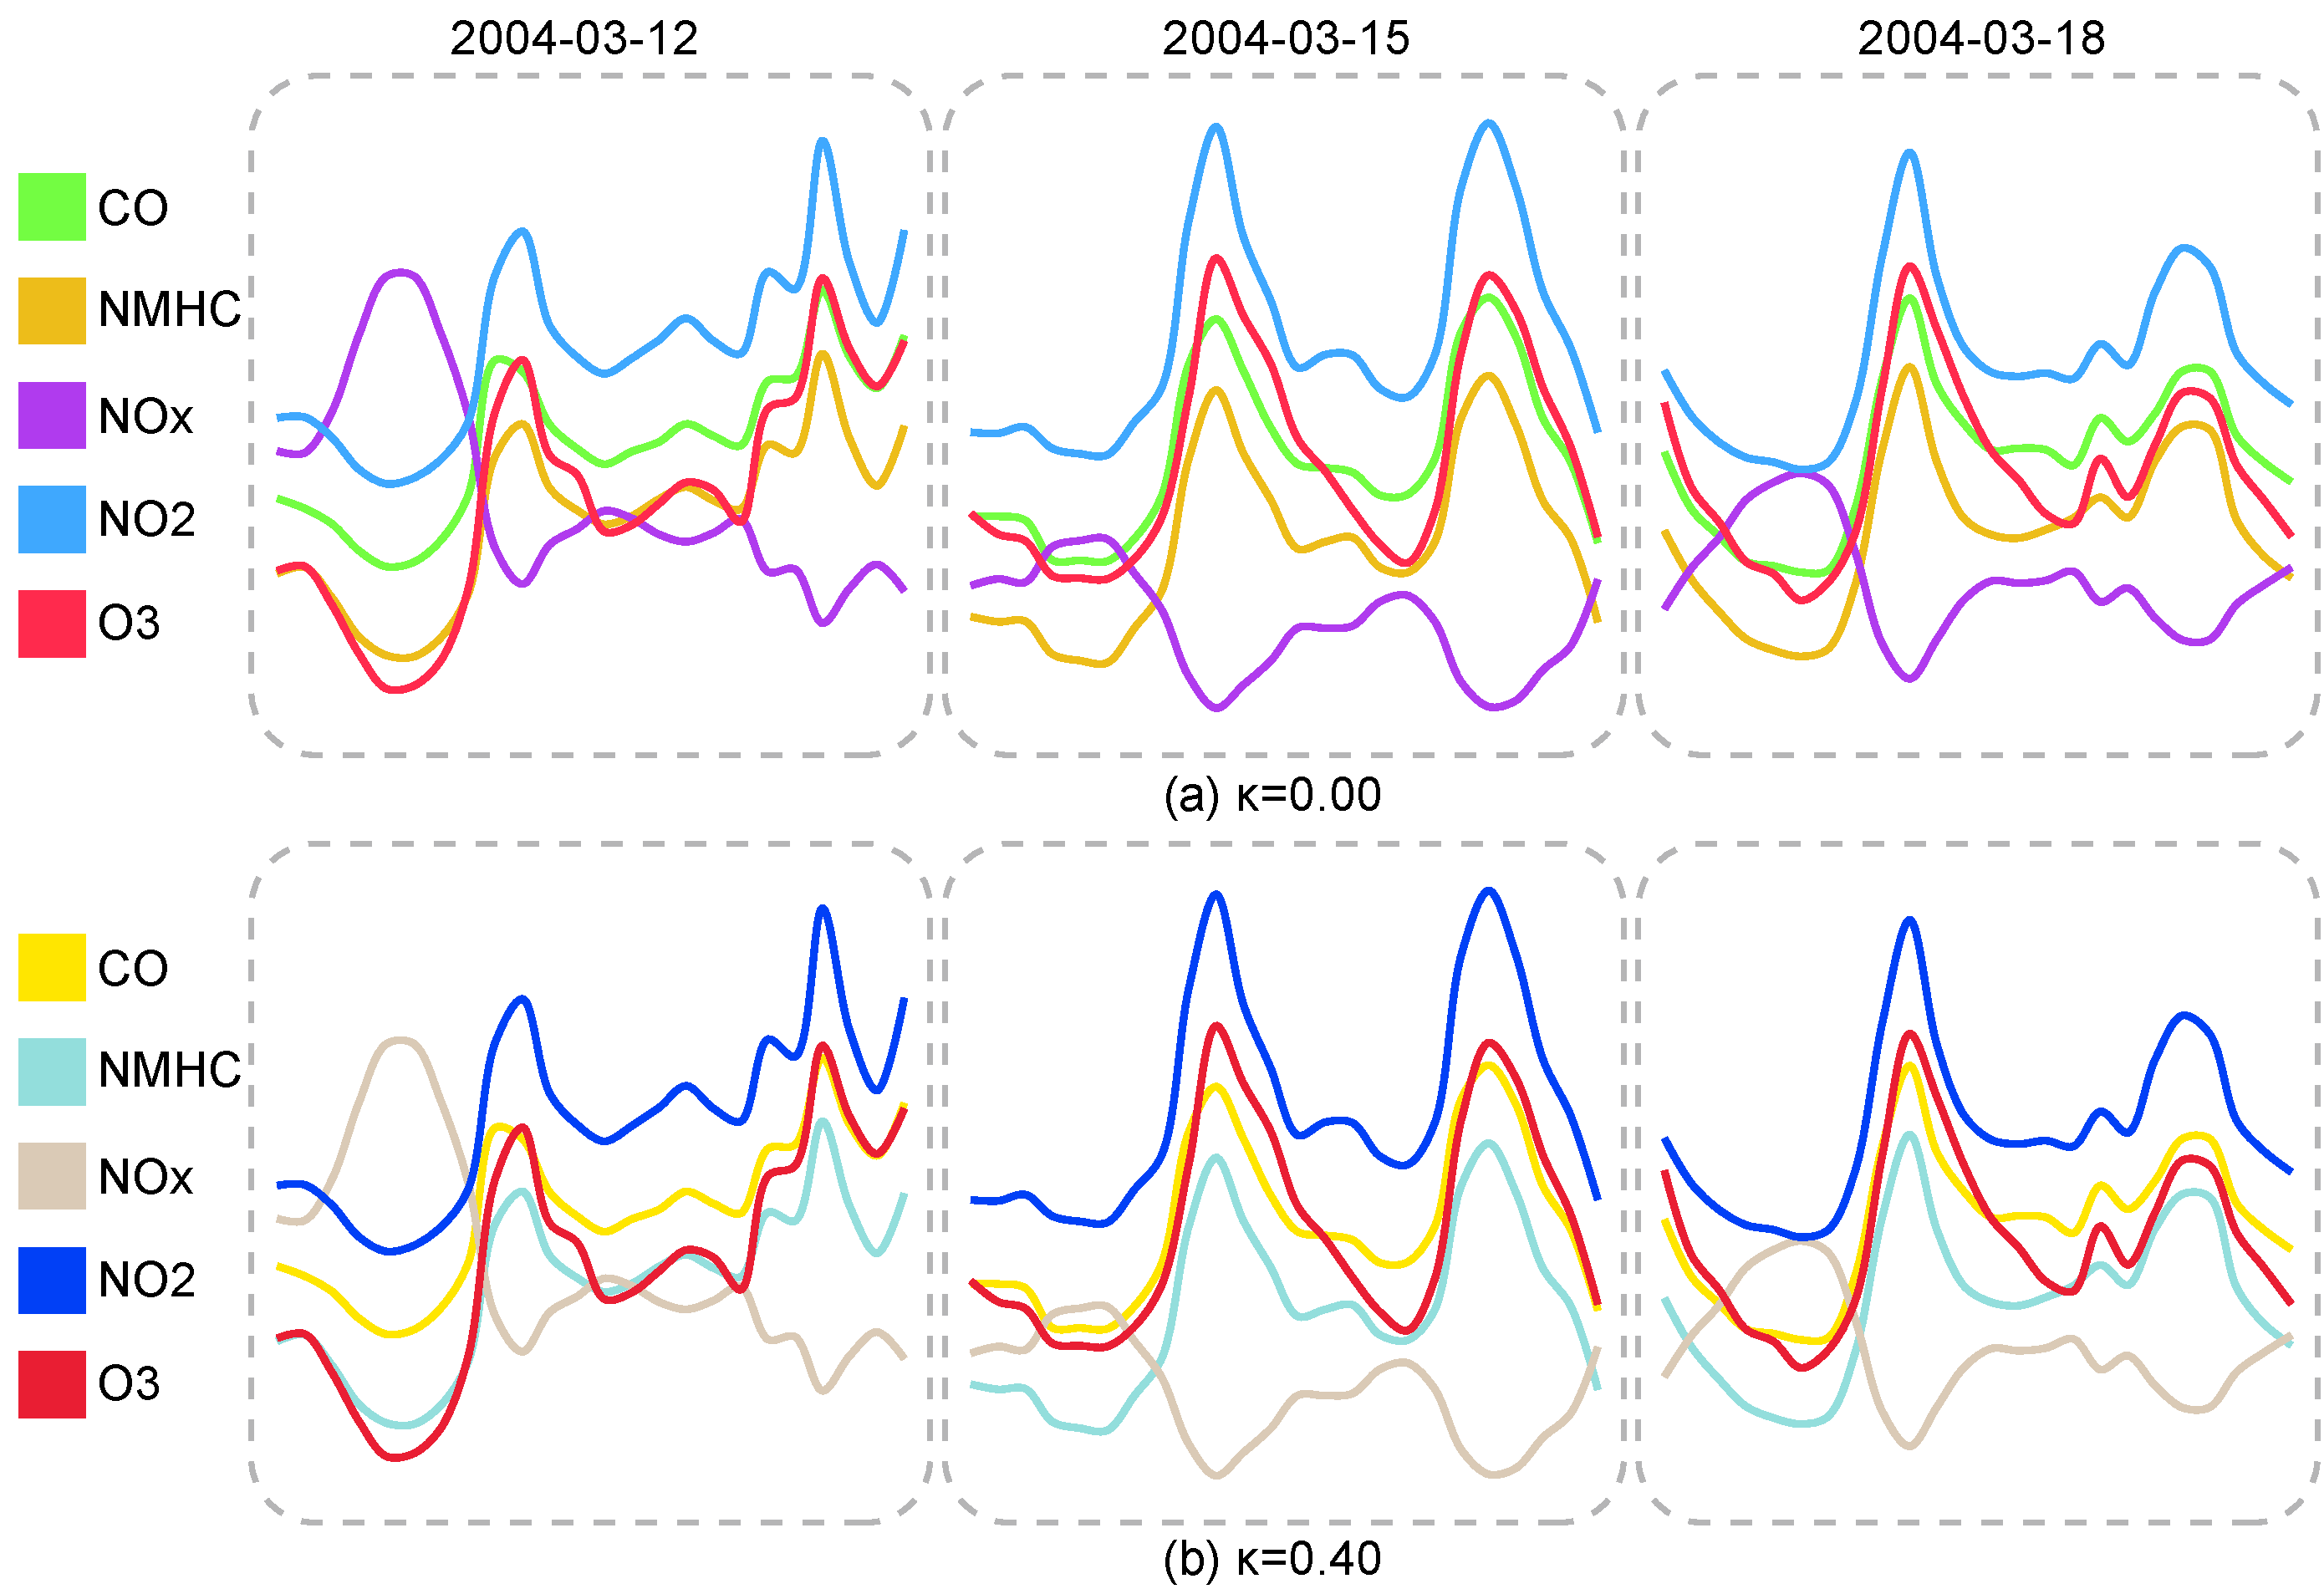
\includegraphics[width=0.96\linewidth]{figures/case-linechart.pdf}
%\caption{Exploring the changes of gases in an air quality data set~\cite{DEVITO2008750}. (a) The automatic generated palette creates salient colors for  all lines. (b) Two selected lines are popping out from the other lines in three views.}
%\vspace*{-3mm}
%\label{fig:caseStudy2}
%\end{figure}

To shed further light onto the ecological validity of our approach, we conducted a case study on a real-world categorical dataset visualized with line charts.
Here, we analyze an air quality data set ~\cite{DEVITO2008750} that contains hourly responses of a gas multi-sensor device deployed in an Italian city from March 12 to March 18, 2014.
The top in Fig.~\ref{fig:ui-case}(b) shows the juxtaposed line graphs encoded by our generated color palette, where each gas type is represented by a line with a unique color.
We can see that all gases are encoded with highly salient colors, making it hard to explore changes of specific gases. This is reasonable because the default $\kappa$ is zero, but all gases have large changes.
Thanks to our interaction mechanism, users can directly select classes of interest to be highlighted by assigning them with large importance, while  the $\theta$ values of the other classes are set to -1. Using the color name constrained palette generation method, the produced palette lets the selected lines pop out from the others (see the bottom in Fig.~\ref{fig:ui-case})). Hence, users can easily explore the changes of the selected two gases (NO$_2$ and O$_3$) in the three juxtaposed views.



%%\section{Discussion \& Future Work}



\bpstart{Mark Attributes}
Our comparison-driven color palettes \textit{guide} viewers' perceptions of the classes with large differences from horizontally juxtaposed visualizations without \textit{enforcing} the difference.
Our study shows that a proper palette can improve the perceptual precision of visual comparisons, whereas mark orientation~\cite{liu2021data} and mark size~\cite{smart2019measuring} both might  have the effect. Note that the number of marks only influences the time for computing contrast measures without the quality of the generated palettes. The reason is that our contrast value is built on nearest neighbourhood graphs, which takes into account the visual density. Even the large datasets with multiple cases at the same position, our generated palettes still perform well.


   
\bpstart{Design Alternatives}
There are a few alternatives for visual comparison~\cite{Gleicher11}.  
Plotting difference between two data series is a clear way~\cite{Gleicher11} to indicate the item with the largest difference. However, it results in that other information  relevant to the data (such as the absolute values) may be absent. Moreover, it is hard to define and visualize the difference between two scatterplots in a meaningful way. 
In contrast, plotting multiple classes with facets~\cite{wickham2009elegant} can help for comparing all categorical visualizations. However, it requires large space when the number of classes is large. We will study and compare the effectiveness of different methods for comparing data with different sizes.


\section {Color Blindness}



Our work concentrated on juxtaposed comparisons to detect changes between multiple datasets, whereas its optimal color palette might not be appropriate for understanding other analytical comparison tasks (e.g., the correlation tasks~\cite{Ondov19}. Future work needs to investigate the effectiveness and extensions of our approach for such comparison tasks. Furthermore, our approach produces colors with salient hue to highlight classes with large changes, but those colors do not visually indicate the ranking of class changes.
It would be helpful to associate the color ordering constraint~\cite{Bujack18} with the degree of changes, so that the ranking of class changes can be shown clearly.


Second, while we only studied the interaction effect between change magnitude and different colorization methods, we plan to investigate how this effect is influenced by different types of changes, such as point number, center position and shape.
The order of rendering is critical for comparison task and we treat it simply in this paper by rendering less important classes first. But when there are multiple important large classes at same positions, the less important class might be overlapped and hard to distinct. Thus a professional render order algorithm is necessary for multi-class scatterplot rendering.

Last, our study only evaluated the effectiveness of our palettes with horizontal juxtaposed visualizations, while there are a few different layout methods such as vertical arrangement, mirrored arrangement, overlaid, and animation. Previous studies~\cite{Ondov19} show that animation performs well in identifying the largest difference and we will conduct studies to learn how well our palette works in this setting.




\bpstart{Study Limitation}

\section {Conclusion and Future Work}
We presented $C^3$-palette, a data-aware approach for producing color
palettes for comparing horizontally juxtaposed categorical visualizations that allows a better identification of the biggest change between two data series, while maintaining the visual discrimination of classes. This goal is
achieved by a  novel co-saliency model, which characterizes the most co-salient features between juxtaposed labeled data visualizations while maintaining class discrimination in the individual visualizations. We evaluated $C^3$-palette through a crowd-sourcing study, which empirically demonstrates that our produced
palettes allow for an efficient visual comparison and good class discrimination.

Our work concentrated on juxtaposed comparisons to detect changes between multiple datasets, whereas its optimal color palette might not be appropriate for understanding other analytical comparison tasks (e.g., correlation tasks, rf.~\cite{Ondov19}. Future work needs to investigate the effectiveness and extensions of our approach for such comparison tasks. Furthermore, mark shape~\cite{liu2021data} and mark size~\cite{smart2019measuring}  might have an effect on the perceptual precision of visual comparisons and we will explore the possibility to model the influence of these factors. %In contrast, the number of marks only influences the efficiency for computing co-saliency, since our co-saliency is based on the nearest neighbourhood graphs built in the data space.

%Even the large datasets with multiple cases at the same position, our generated palettes still perform well.

Second, our approach produces colors with salient hue to highlight classes with large changes, but those colors do not visually indicate the ranking of class changes. It would be helpful to associate a color ordering constraint~\cite{Bujack18} with the degree of changes, so that the ranking of class changes can be shown clearly. On the other hand, our method can be extended to generate palettes for people with color vision deficiency by incorporating a physiologically-based model~\cite{machado2009physiologically} into our optimization framework.

Third, while our second user study only examined the interaction effect between change magnitude and different colorization methods, we plan to investigate how this effect is influenced by different types of changes in scatterplots, such as point number, center position and shape.
The order of rendering is critical for the comparison task and in this paper we treat it simply by rendering less important classes first. But when there are multiple important large classes at the same positions, less important classes might be overlapped and hard to distinguish. Thus a professional render order algorithm would be necessary for multi-class scatterplot rendering.

Last, our study only evaluated the effectiveness of our palettes with horizontally juxtaposed visualizations, while there are different layout methods such as vertical arrangement, mirrored arrangement, overlaid, and animation. Previous studies~\cite{Ondov19} show that animation performs well in identifying the largest difference and we will conduct studies to learn how well our palette works in this setting. On the other hand, there are a few 
different visual comparison methods~\cite{Gleicher11} such as plotting differences and faceting groups~\cite{wickham2009elegant}. It would be helpful to fully investigate the strengths and limitations of each of these methods for visual comparisons.




%%
%% The acknowledgments section is defined using the "acks" environment
%% (and NOT an unnumbered section). This ensures the proper
%% identification of the section in the article metadata, and the
%% consistent spelling of the heading.
%\begin{acks}
%To Robert, for the bagels and explaining CMYK and color spaces.
%\end{acks}

%%
%% The next two lines define the bibliography style to be used, and
%% the bibliography file.
\bibliographystyle{ACM-Reference-Format}
\bibliography{coSaliency}

\end{document}
\endinput
%%
%% End of file `sample-authordraft.tex'.
